\newif\ifpagetuning

\pagetuningtrue % trying to get page breaks in the best spots

\newif\ifnotcutting \notcuttingtrue % set if not cutting down to size

\newif\iffinaldraft \finaldrafttrue % true if it's the final version

\newif\iftimestamp\timestamptrue  % show MD5 stamp of paper

% \timestampfalse % it's post-submission time

\newcommand\vfilbreak[1]{\vskip 0pt plus #1 \penalty-200 \vskip 0pt plus -#1 }


\IfFileExists{timestamp.tex}{}{\timestampfalse}

\newif\ifpdfmadness


\ifx\pdfoutput\undefined
   \pdfmadnessfalse
\else
   \ifnum\pdfoutput=1
     \pdfmadnesstrue
   \else
     \pdfmadnessfalse
   \fi
\fi

\ifpdfmadness
  \def\loadpdf[#1]#2{\includegraphics[#1]{#2.pdf}}
\else
  \def\loadpdf[#1]#2{\includegraphics[#1]{#2.eps}}
\fi



\documentclass[]{jfp1}

\newcommand\mrfy{MRFy} % damn you Noah

\newcommand\txprobj[3][]{a#1_{{#2}_{j-1}{#3}_j}} % probability entering j
\newcommand\txprobxj[3][]{a#1_{{#2}_{j}{#3}_{j+1}}}  % probability exiting j
\newcommand\txprobjj[3][]{a#1_{{#2}_{j}{#3}_j}} % probability within j
\newcommand\alignwidth{\ensuremath C} % number of columns in an alignment
\newcommand\pairedwith[1]{{\pi(#1)}}

\newcommand\primcons{\texttt{\small(:)}}

\ifpagetuning
  \newcommand\tuningbox{\vbox}
\else
  \newcommand\tuningbox{\relax}
\fi

\newcommand\naive{na\"\i ve}
\usepackage{url}
%\usepackage{amsmath}
\usepackage{array}
\usepackage{listings}
\usepackage{graphicx}
\lstset{
    tabsize = 2,
    basicstyle = \ttfamily,
    language = Haskell
    }    

\newcommand\figref[1]{Figure~\ref{fig:#1}}
\newcommand\figrefpair[3][and]{Figures \ref{fig:#2}~#1~\ref{fig:#3}}
\newcommand\figlabel[1]{\label{fig:#1}}
\newcommand\secref[1]{Section~\ref{sec:#1}}
\newcommand\secrefpair[3][and]{Sections \ref{sec:#2}~#1~\ref{sec:#3}}
\newcommand\seclabel[1]{\label{sec:#1}}

\usepackage{verbatim}

\newif\ifverbatimsmall
\verbatimsmallfalse
\makeatletter
\def\verbatim@font{%
   \normalfont\ttfamily
   \ifverbatimsmall\small\fi
   \hyphenchar\font\m@ne
   \@noligs}
\newcommand{\mono}[1]{%
  {\@tempdima = \fontdimen2\font
   \texttt{\spaceskip = 1.1\@tempdima #1}}}
\makeatother

\newskip\presvtopsep

\newenvironment{smallverbatim}{\par\small\verbatimsmalltrue\verbatim}{\endverbatim}
\newcommand\smallverbatiminput[1]{%
  \verbatimsmalltrue
  \presvtopsep=\topsep
  \topsep=0.78\topsep
  \verbatiminput{#1}%
  \verbatimsmallfalse
  \topsep=\presvtopsep
}
\newcommand\smallfuzzverbatiminput[2]{%
  \hfuzz=#1 \smallverbatiminput{#2}\hfuzz=0pt }

\renewcommand\ttdefault{aett}

  \long\def\remark#1{%
      \ifvmode
         \marginpar{\raggedright\hbadness=10000
         \parindent=8pt \parskip=2pt
         \def\baselinestretch{0.8}\tiny
         \itshape\noindent #1\par}%
      \else
          \unskip\raisebox{-3.5pt}{\rlap{$\scriptstyle\diamond$}}%
          \marginpar{\raggedright\hbadness=10000
         \parindent=8pt \parskip=2pt
         \def\baselinestretch{0.8}\tiny
         \itshape\noindent #1\par}%
      \fi}

\iffinaldraft
  \newcommand\finalremark{\remark}
\else
  \newcommand\finalremark[1]{\relax}
\fi


\usepackage[authoryear]{natbib}
\bibpunct();A{},
\let\cite\citep
\let\citeyearnopar=\citeyear
\let\citeyear=\citeyearpar

\renewcommand\bibsection{\section*{\refname}}



\IfFileExists{timestamp.tex}{\input{timestamp}}{}
\renewcommand{\floatpagefraction}{0.9} % must be less than \topfraction
\renewcommand{\topfraction}{0.95}
\renewcommand{\textfraction}{0.05}

\title{Haskell in Computational Biology}

\author[N. M. Daniels, A. Gallant, and N. Ramsey]
        {Noah M. Daniels, Andrew Gallant, and Norman Ramsey \\
           {Department of Computer Science, Tufts University}\\
           {\email{{\rmfamily\{}ndaniels, agallant, nr{\rmfamily\}}@cs.tufts.edu}}}


\begin{document}

\overfullrule=10pt


\iftimestamp
%\preprintfooter{\mdfivestamp} 
\fi


\maketitle

%
% It can't hurt to remind everyone involved exactly what an Experience
% Report is.
%
%
\begin{abstract}
%An Experience Report provides {evidence} that functional
%programming really works, or it describes obstacles that prevent
%functional programming from working.   
Haskell gives computational biologists
the flexibility and rapid prototyping of a scripting
language, and it compiles to native code.
From experience using Haskell to implement new algorithms for
computational biology, we~report where Haskell really worked for us
and what obstacles prevented it from working better.
Higher-order functions, lazy evaluation, and
monads worked well, but
profiling and debugging presented obstacles.
And~because allocation costs are difficult to predict and control,
compilation to native code did not guarantee great performance.
Finally, our experience with Haskell libraries varied greatly:
memoization combinators and parallel-evaluation
strategies helped us a lot,
but other, nameless libraries mostly got in our way.
Despite the obstacles and the uncertain quality of some libraries,
Haskell's ecosystem
made it easy for us to explore and run new algorithms.
\end{abstract}


\section{Introduction}

Computational biologists write software that answers questions about 
sequences of nucleic acids (genomic data) or sequences of amino 
acids (proteomic data). 
When performance is paramount,
software is usually written in C~or~C++. 
When convenience, readability, and
productivity are more important,
software is usually written in a dynamically typed
or domain-specific language like
Perl, Python, Ruby, SPSS, or~R.
In~this paper, we report on experience using a third kind of language,
Haskell.
Although we encountered some obstacles that kept Haskell from working
as well as we would have liked, our overall experience was positive:
Haskell really worked for us, and we believe it will work equally well
for other computational biologists.
\begin{itemize}
\item
We had to reimplement an
algorithm already implemented in~C++, 
and the Haskell code is slower.
But the Haskell code was easy to write,     % coherent subject!
clearly implements the underlying mathematics
 (\secref{viterbi}),
 was easy to parallelize,
and performs well enough
(\secref{perf}).
  And our new tool solves a problem that could not be solved by
  the~C++ tool which preceded~it.
\item
Higher-order functions made it unusually easy to
create and experiment with new stochastic-search algorithms
(\secref{hofs}).
\item
Haskell slowed us down in only one area:  understanding and
improving
performance (\secrefpair{improving-viterbi}{awkward-profiling}).
%%  \item
%%  The only significant impediment that Haskell presented to our
%%  research was the difficulty of understanding and improving the
%%  performance of Haskell programs (\secref{awkward-profiling}).
\item
Although the first two authors are computational
biologists
with little functional-programming experience,
Haskell made it easy for us to explore new research ideas.
By~contrast,
our group's C++ code has 
made it hard to explore
% been a good vehicle for exploring 
new ideas
(\secref{comparo}).
\item
The Haskell community offers libraries and tools that
promise powerful abstractions.
Some kept the promise, saved us lots of effort, and were a pleasure
to~use.
Others, not so much.
We couldn't tell in advance which 
would be which
 (\secref{penumbra}).
\end{itemize}
A~preliminary version of this
paper \citep{daniels:haskell-in-bio:2012} was presented as 
an \emph{Experience Report} in ICFP~2012.
This~paper adds a new technical section (\secref{improving-viterbi})
which describes our experience 
refactoring and improving our implementation of Viterbi's 
\citeyearpar{Viterbi:1967hq}
algorithm.
We~have also simplified the stochastic search as well as other elements of
the code.
Finally, we~have improved and added to explanations, figures, and diagrams.




\section{The biology}

Proteins, by
interacting with one another and with other 
molecules, carry out the functions of living cells: metabolism, regulation, 
signaling, and so on.
A~protein's function is determined by its structure, 
and its structure is determined by the sequence of amino acids that
form the protein.
The amino-acid sequence is ultimately determined by a sequence of
nucleic acids in DNA, which we call a gene.
Given a gene, biologists wish to know the cellular
function of the protein the gene codes for.
One of the best known methods of discovering such function is
to find other proteins of 
similar structure, which likely share similar function.
Proteins that share structure and function are expected to be
descended from a common ancestor---in biological terms, \emph{homologous}---and
thus
the problem of identifying proteins similar to a \textit{query sequence} is called 
\textit{homology detection}.




Computational biologists detect homologies by building 
algorithms which, given a {query sequence}, %% of amino acids,
compare it with known proteins.
When the known proteins have amino-acid sequences that
are not too different from the query sequence, homology can be
detected by
a family of algorithms called 
\textit{hidden Markov models}~\cite{Eddy:1998ut}.
But in real biological systems,
proteins with similar structure and function may be formed from significantly 
different amino-acid sequences, which are not close in edit distance.
Our~research software, MRFy (pronounced
``Murphy''), can detect homologies 
in amino-acid sequences that are only distantly related.

A~paper for the computational biology community, based on MRFy, has been
submitted to the ACM Conference on Bioinformatics, Computational Biology, and 
Biomedical Informatics.
That paper explores the effectiveness of various search strategies,
and it also
compares MRFy with several other software tools.
MRFy is more accurate than the other software tested.
MRFy is available at \url{mrfy.cs.tufts.edu}.
%
%We will explain an 
%algorithm for detecting reasonably similar sequences, and then move on to 
%explain MRFy, our novel approach for detecting more distantly related sequences 
%for proteins that share similar structure and function.
%

%
% I hope the new intro renders these two sentences unnecessary. ---NR
%
%
%%  
%%  To~enable you to understand our experience with Haskell,
%%  we~sketch not only the MRFy algorithm (\secref{mrfy})
%%  but also one of the older hidden-Markov algorithms (\secref{viterbi}),
%%  which is incorporated into~MRFy.


\section{The software}



Homology-detection software is most often used in one of two ways:
to test a hypothesis about 
the function of a single, newly discovered protein, or 
to compare every protein in a genome against a library of known protein 
structures.
Either way, 
the software is \emph{trained}
on a group of proteins that share function and structure.
These proteins are identified by a biologist, who puts
their amino-acid sequences into an
\emph{alignment}. 
This alignment relates individual amino acids in a set of homologous proteins.
An~alignment may be represented as a matrix
in which each row corresponds to the amino-acid sequence of a protein,
and each column groups amino acids that play similar roles in
different proteins (\figref{alignment}).


An alignment may contain \emph{gaps}, which in 
\figref{alignment} are shown as dashes.
A~gap in row~2, column~$j$ indicates that as proteins evolved, either 
protein~2 lost its amino acid in position~$j$, or 
other proteins gained an amino acid in position~$j$.
If~column~$j$ contains few gaps, 
it~is considered a \emph{consensus column},
and the few proteins with gaps probably lost amino acids via
\emph{deletions}.
%%  \remark{NMD: Missing is the fact that all these models
%%  are directionless; they don't care whether something was gained or lost
%%  over time. But this doesn't matter.}
If~column~$j$ contains \emph{mostly} gaps, 
it~is considered a \emph{non-consensus column},
and the few proteins without gaps probably gained amino acids via
\emph{insertions}. 


Once a protein alignment is constructed, it~is used to train a
\emph{hidden Markov model}. 
A~hidden Markov model is a probabilistic finite-state machine which 
can assign a probability to any query sequence.
A~protein whose query sequence has a higher probability is more likely to %
be homologous to the proteins in the alignment.
We~write a query sequence as $x_1, \ldots, x_{\scriptscriptstyle N}$,
where each $x_i$~is 
an amino-acid \emph{residue}.\footnote
{When an amino acid combines with other amino acids to form a protein, it gives up
two hydrogen atoms and an oxygen atom.
What's left is called
a \emph{residue}.
In~this paper we use the terms ``residue'' and ``amino acid'' 
interchangeably.
}
The number of residues, $N$, can differ from the number of columns
in the alignment,~\alignwidth. 


\begin{figure}
\ifpdfmadness
\centerline{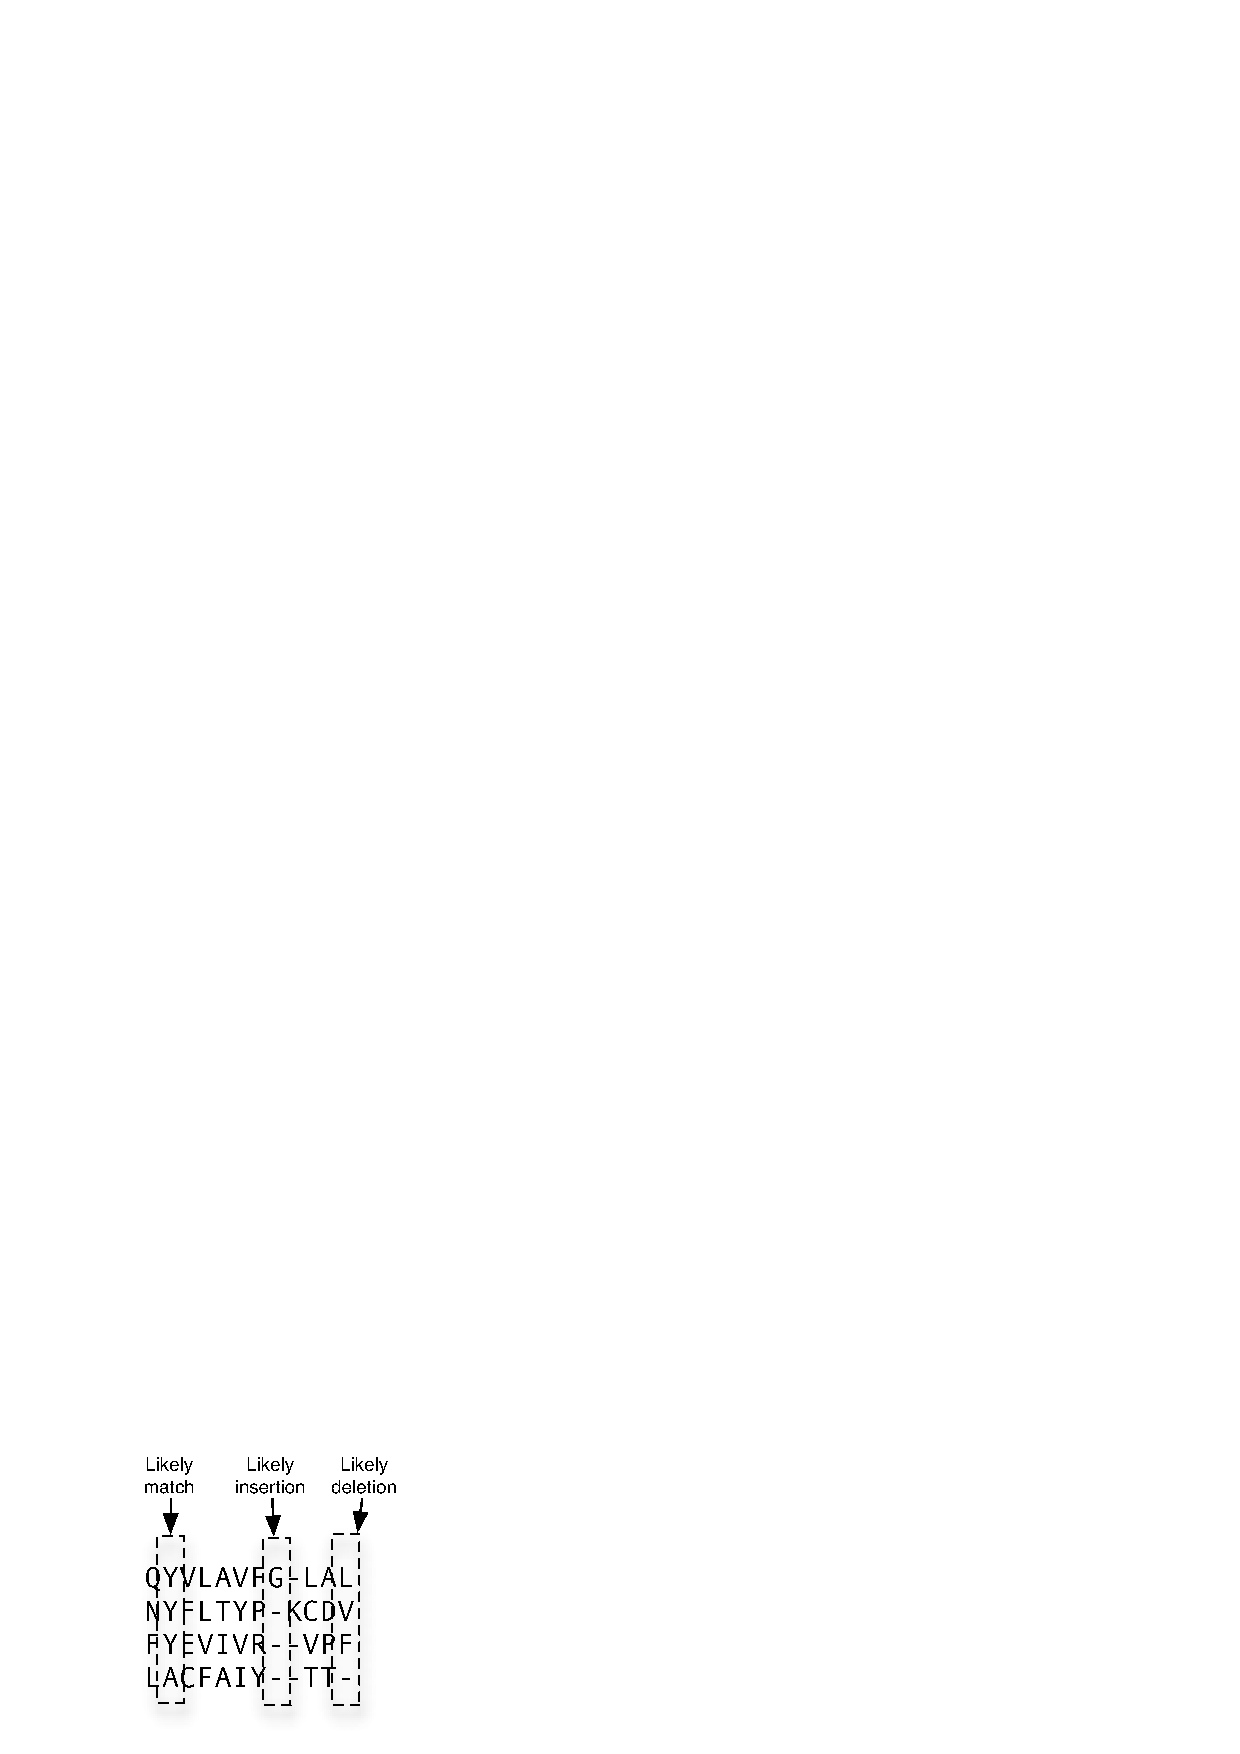
\includegraphics[width=8cm]{alignment.pdf}} 
\else
\centerline{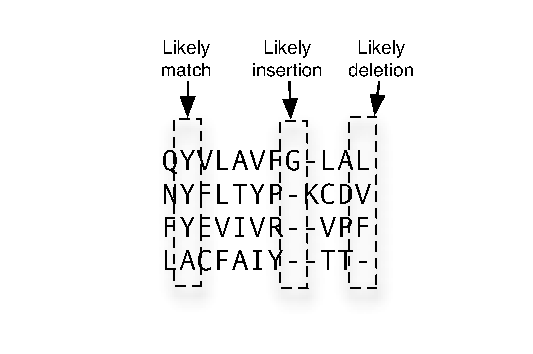
\includegraphics[width=8cm]{alignment.eps}} 
\fi

\caption{A~structural alignment of four proteins $(\alignwidth = 12)$}
\figlabel{alignment} 
\end{figure}



A~hidden Markov model carries probabilities on some states and on all
state transitions.
Both the probabilities and the states are determined by the alignment:
\begin{itemize}
\item
For each column~$j$ of the alignment, the hidden Markov model has a
\emph{match state}~$M_j$.
The match state contains a table $e_{M_j}(x)$ which gives the
 probability that a homologous protein has residue~$x$ in
 column~$j$.
\item 
For each column~$j$ of the alignment, the hidden Markov model has an
\emph{insertion state}~$I_j$.
The insertion state contains a table $e_{I_j}(x)$ which gives the
probability that a homologous protein has gained residue~$x$ by
insertion at column~$j$.
\item
For each column~$j$ of the alignment, the hidden Markov model has a
\emph{deletion state}~$D_j$.
The deletion state determines the probability that a homologous protein
has lost a~residue by deletion from column~$j$.
A~deletion state contains no tables of probabilities.
\hfuzz=1.5pt % fix blot
\end{itemize}
The probabilities $e_{M_j}(x)$ and $e_{I_j}(x)$ are \emph{emission probabilities}.
The names of the states are easily confused;
one~way to keep them straight is to imagine that the model of the
alignment describes a prototype sequence of length~$\alignwidth$,
and that each state describes an action used to build the query
sequence from the prototype: 
match a prototypical residue,
insert an unexpected residue,
or
delete a prototypical residue.


A~hidden Markov model also has distinguished ``begin'' and ``end''
states; begin and end states are like match states, but they
correspond to no residues and contain no emission probabilities.
%%
%% for consistency with the text above 'begin' and 'end' are neither
%% capitalized nor italicized.
%%
In~our representation, 
the begin and end states are known by their positions:
in a $\alignwidth$-column model, the begin state shares
column~0 with an insertion state, and the end state is the only state
in column~$\alignwidth$. 
Every other state is referred to by its column~$j$
and by one of these labels:\label{code:state-label}
\smallverbatiminput{statelabel}
We~group states that share a column~$j$; these states are referred
to collectively as ``node~$j$,'' as shown in \figref{plan7}.
This model
has begin and end states $B$~and~$E$;
an~insertion state in node~0; and
four
full nodes, each containing 
an insertion state~$I$, 
a match state~$M$, and a
deletion state~$D$.
(Node~0 may also be viewed as a full node, but its deletion state is
not reachable from the begin state, so it is shown with only two
states.) 

\begin{figure} 
\centerline{\loadpdf[width=11cm]{Plan7_emit}} 

\caption{A hidden Markov model $(\alignwidth = 4)$}

\figlabel{plan7}
\end{figure}

The model in \figref{plan7} is from a well-established family
that permits
transitions between match states and all other adjacent states,
but forbids
direct
transitions between insertion 
states and deletion states  \cite{Eddy:1998ut}. 
Models in this family are called ``Plan7'' models because
every full node has 7~transitions.
Each transition has its own probability; the probabilities for
transitions leaving states in node~$j$ are
$\txprobjj I I$,
$\txprobxj I M$,
$\txprobjj M I$,
$\txprobxj M M$,
$\txprobxj M D$,
$\txprobxj D M$,
and
$\txprobxj D D$.
(The transitions from match to insertion and from insertion to
insertion leave states in 
node~$j$ but also enter states in node~$j$.
The other transitions enter states in node~$j+1$.)
When column $j+1$ is a consensus column, transitions that enter
its match state 
%($\txprobxj I M$,
%$\txprobxj M M$,
%$\txprobxj D M$)
are more likely.
When column $j+1$ is a non-consensus column, transitions that enter
its insertion and deletion states are more likely.








\subsection{Computing probabilities using perspicuous Haskell}

\seclabel{viterbi}


Given a hidden Markov model, 
an~established software package called HMMER (pronounced ``hammer'') 
can compute the probability
that a new protein shares structure 
with the proteins used to train the model.
The computation finds the most likely matching path through the hidden Markov model.
In~any matching path, each match state and insertion state corresponds to a
unique residue in the query sequence.
The probability of the path is the product of all of the corresponding
emission probabilities, together with the product of the transition
probabilities along the edges of the path.

Probabilities are small, and products of small numbers can become very
small indeed.
If~we were to multiply probabilities represented as floating-point
numbers, all the useful information would wind up in exponents,
and an exponent holds only
11~bits.
In~order to store useful information in the significand, which holds 53~bits,
we~follow standard practice: instead of multiplying probabilities,
we~add logarithms of probabilities \cite{Viterbi:1967hq}.
Also following standard practice, we~work with
\emph{negated}
logarithms of probabilities, which are  positive numbers.
The negated logarithm of a probability is called a \emph{score}:
\smallverbatiminput{score}
We~have given type \texttt{Score} a limited \texttt{Num} instance which permits
scores to be added and subtracted but not multiplied.


\def\goo{18pt}
\def\gum{14pt}
\newcommand\vsum[2]{#2&{}+{}& #1}

\begin{figure}
  
%%  \[
%%  \def\maxiquad{\hskip 1.2em\relax}
%%  %\mskip -5mu
%%  \begin{array}{@{}l@{}c@{}l}
%%  V_{j}^{M}(i) &{}={}& \log\frac{e_{M_{j}}(x_{i})}{q_{x_{i}}} + \max \left\{
%%    \begin{array}{l@{}c@{}l}
%%    \vsum{V_{j-1}^{M}(i - 1)} {\log a_{M_{j-1}M_{j}}}\\
%%    \vsum{V_{j-1}^{I}(i - 1)} {\log a_{I_{j-1}M_{j}}}\\
%%    \vsum{V_{j-1}^{D}(i - 1)} {\log a_{D_{j-1}M_{j}}}\\
%%    \end{array} \right.\\[\goo]
%%  V_{j}^{I}(i) &=& \log\frac{e_{I_{j}}(x_{i})}{q_{x_{i}}} + \max \left\{
%%    \begin{array}{l@{}c@{}l}
%%    \vsum{V_{j}^{M}(i - 1)} {\log a_{M_{j}I_{j}}}\\
%%    \vsum{V_{j}^{I}(i - 1)} {\log a_{I_{j}I_{j}}}\\
%%    \end{array} \right.\\[\gum]
%%  V_{j}^{D}(i) &=& \max \left\{
%%    \begin{array}{l@{}c@{}l}
%%    \vsum{V_{j-1}^{M}(i)} {\log a_{M_{j-1}D_{j}}}\\
%%    \vsum{V_{j-1}^{D}(i)} {\log a_{D_{j-1}D_{j}}}\\
%%    \end{array} \right.\\
%%  \end{array}
%%  \]
%%  
%%  \caption{Viterbi's original equations}
%%  \figlabel{viterbi-original}
%%  
%%  
%%  \bigskip

%\begin{figure}
\[
\begin{array}{l@{}c@{}l@{}}
V_{j}^{\prime M}(i) &{}={}& e^{\prime}_{M_{j}}(x_{i}) + \min \left\{
  \begin{array}{l@{}c@{}l}
  \vsum{V_{j-1}^{\prime M}(i - 1)} {a^{\prime}_{M_{j-1}M_{j}}}\\
  \vsum{V_{j-1}^{\prime I}(i - 1)} {a^{\prime}_{I_{j-1}M_{j}}}\\
  \vsum{V_{j-1}^{\prime D}(i - 1)} {a^{\prime}_{D_{j-1}M_{j}}}\\
  \end{array} \right.\\[\goo]
V_{j}^{\prime I}(i) &=& e^{\prime}_{I_{j}}(x_{i}) + \min \left\{
  \begin{array}{l@{}c@{}l}
  \vsum{V_{j}^{\prime M}(i - 1)} {a^{\prime}_{M_{j}I_{j}}}\\
  \vsum{V_{j}^{\prime I}(i - 1)} {a^{\prime}_{I_{j}I_{j}}}\\
  \end{array} \right.\\[\gum]
V_{j}^{\prime D}(i) &=& \min \left\{
  \begin{array}{l@{}c@{}l}
  \vsum{V_{j-1}^{\prime M}(i)} {a^{\prime}_{M_{j-1}D_{j}}}\\
  \vsum{V_{j-1}^{\prime D}(i)} {a^{\prime}_{D_{j-1}D_{j}}}\\
  \end{array} \right.\\[\gum]
%
\multicolumn3{l@{}}{%
  a'_{s \hat{s}} = - \log a_{s \hat{s}} 
\qquad
  e^{\prime}_{s}(x) = - \log\frac{e_{s}(x)}{q_{x}}
\qquad
  V_j^{\prime M}(i) = - V_j^{M}(i)
}
\\
\end{array}
\]

\caption{Viterbi's equations expressed using scores}
\figlabel{viterbi-transformed}
\end{figure}




\ifpagetuning\enlargethispage{1.2\baselineskip}\fi


The~most likely path through a model is the one with the
smallest score.
The~score of each path is computed by dynamic programming; the score associated with
a path to a state~$s$ ($M$, $I$, or~$D$) at node~$j$ and position~$i$ in
the query sequence is written $V_j^{\prime s}(i)$.
For~example, 
score~$V_j^{\prime M}(i)$ represents the probability of the most
likely path of the first $i$~residues in the query sequence,
terminating with placement of residue~$x_i$ in state~$M_j$.
Scores $V_j^{\prime I}(i)$~and~$V_j^{\prime D}(i)$ are similar.
Scores are specified by Viterbi's equations, which are shown
in \figref{viterbi-transformed}. 
The~equations (expressed using probabilities) are explained very clearly by
\citet[Chapter~5]{Durbin:1998wz}


To~use Haskell, we had to reimplement the standard
algorithm for solving Viterbi's equations.
Haskell made it possible for us to write code that looks like the
math,
which made the code easy to write and gives us confidence that it is
correct.

Our code represents a query sequence as an immutable array of residues.
In~idiomatic Haskell, 
we might represent an individual residue~$x_i$
using a value of algebraic data type with constructors named for
amino acids:
\begin{smallverbatim}
data Amino = Ala | Cys | Asp | Glu | ...   -- not used
\end{smallverbatim}
But in our
legacy file format, each amino acid (residue) is a small integer
used only to index arrays.
%which we use only as an array index.
We therefore chose a representation that is easier to make consistent
with query sequences as represented on~disk:
\smallverbatiminput{aa}

%%  \remark{I'm not sure if this is the whole story, since the reader might simply
%%    ask, ``Why not map 0 to Ala, 1 to Cys, etc.?''. The real reason we keep the
%%    ``Int'' here I think, is that it provides easy indexing into the match and
%%    insertion emission vectors.}



A~model is represented as a sequence of \emph{nodes}, 
each of which includes three states:\label{code:model3-node}
\smallverbatiminput{model3-node}
The representation of a state~$s$ includes the scores of transitions leaving
that state;
if~state~$s$ is a match or insertion state, its representation also
includes a table of emission scores.
For~example, the representation of a match state is \texttt{MState}:
\smallverbatiminput{model3-mstate}
%
The transition scores, which are shown as $a_{s\hat s}$
in \figref{plan7}, are read by  
function \texttt{aScore}, 
%which is given states $s$~and~$\hat s$ and a node index~$j$; its
whose
specification is
\mbox{$\mathtt{aScore}\;s\;\hat s\;j = \txprobxj s {\hat s}$}.\seclabel{aScore}
The
emission table is read by 
\texttt{eScore}, whose specification
is % parallel structure for line breaking below
\mbox{$\mathtt{eScore}\;s\;j\;i = e'_{s_j}(x_i)$},
where $x_i$ is the residue located at position~$i$ in the query
sequence. 
%
%%  We place the transition probabilities 
%%  into a record in which each field is labeled
%%  \texttt{$s$\_$\mskip 1mu\hat s$},
%%  where $s$~and~$\hat s$ form one of the 7~permissible pairs of state
%%  labels:\label{sec:tprobs}
%%  \smallverbatiminput{tprob-tprobs}
%%  \remark{Need to explain those last two fields. HMMer?}

%%  DROP THIS PARA??
%%  Nodes are numbered, and the representation of a node includes 
%%  the tables
%%  of emission probabilities for the match and insertion states,
%%  plus
%%  the
%%  probabilities of transitions 
%%  into the states of that node.
%%  \smallverbatiminput{hmmnode}

All scores computed by \mrfy\ are sums of these transition and
emission scores.
Because these sums can be usefully attached to many types of values,
we~have defined a small abstraction:
\smallfuzzverbatiminput{10.8pt}{vscore}
Think of a value of type \mono{Scored~a} as a container holding
 an~``\texttt a'' with a score written on the side.
%% \remark{Lazy in the first arg is about 1\%~slower}
The \texttt{/+/} function adds to the score without touching the
 container.
Function \texttt{fmap} is also defined; it~applies a function to a
 container's contents. 
%
Finally, we~made \texttt{Scored} an instance of~\texttt{Ord}.
Containers are ordered by score alone, so applying
\texttt{minimum} to a list of scored things chooses the thing with the
smallest (and therefore best) score.


Armed with our models and with the \texttt{Scored} abstraction, we
attacked Viterbi's equations. 
The probability in each state is a function of the probabilities
in its predecessor states, 
and all probabilities can be computed by a classic dynamic-programming
algorithm.
This algorithm starts at the {begin} state,
computes probabilites in nodes $1$~through~$\alignwidth$ in
succession, and terminates at the {end} state.
One of us implemented this algorithm, storing the probabilities in an array.
The cost was
$O(|N|\times|\alignwidth|)$;
in~MRFy, $\alignwidth$~and~$N$ range from several hundred to a few
thousand.



%%  For 
%%  reasons including floating point underflow, the HMMER software (with which we 
%%  maintain file format compatibility) stores all probabilities in a trained HMM 
%%  file as negative natural logs.
%%  Thus, the Viterbi recurrence relations are 
%%  simplified from the form in \ref{viterbi_eqn} to that in \ref{viterbi_log_eqn}, 
%%  and because they are \textit{negative} logs, the problem transforms from 
%%  maximization to minimization.


\seclabel{cons}
\seclabel{vee-prime}


Another of us was curious to try coding Viterbi's equations
directly as recursive functions.
Like a recursive Fibonacci function, Viterbi's functions,
if~implemented \naive ly,
take exponential time.
But like the Fibonacci function, Viterbi's functions can be
\emph{memoized}.
For example, to compute $V_j^{\prime M}(i)$ using the equation at the top
of \figref{viterbi-transformed}, we define
\mbox{\texttt{vee\char`\'} \texttt{Mat} $j$ $i$}.
The equation adds~$e^{\prime}_{M_{j}}(x_{i})$, computed
with \texttt{eScore}, to a minimum of sums.
The~sum of an~$a'_{s\hat s}$~term and a $V^{\prime s}_{j-1}(i-1)$ term 
is computed by function \texttt{avSum}, in which
the terms are computed by \texttt{aScore} and \texttt{vee''},
respectively:\label{code:vee-prime} 
\smallfuzzverbatiminput{2.9pt}{vfix}
%%%%%%%%%% horrible line break
% The right-hand side of \verb+vee'+ is wrapped in a call to
What about the call to
\mono{\mbox{fmap (Mat `cons`)}}?
This call performs a computation \emph{not} shown
in \figref{viterbi-transformed}:
\mrfy\ computes not only the {probability} of the most likely path but 
also the path itself.
Function \mono{(Mat `cons`)} adds~$M$ to a path;
we~avoid \mbox{\mono{(Mat :)}} for reasons explained
in \secref{performance} below. 

Function~\verb+vee'+ makes a recursive call not to itself but
to~\verb+vee''+. 
Function~\verb+vee''+ is the {memoized} version of~\verb+vee'+;
it~produces the same result as~\verb+vee'+,
but repeated calls return in constant time:
\smallverbatiminput{memo}
Functions \texttt{Memo.memo3} and \texttt{Memo.arrayRange} come from
Luke Palmer's
package
\path{Data.MemoCombinators}.
The value
\texttt{numNodes} represents~$\alignwidth$,
and \texttt{seqlen} represents~$N$.

Memoization makes \verb+vee'+ perform as well as our classic
dynamic-programming code.
And~the call to \texttt{Memo.memo3} is the \emph{only} part of the code
devoted to dynamic programming.
By~contrast, standard implementations of Viterbi's algorithm, such as in HMMER,
spend much of their code 
managing dynamic-programming tables.
Haskell enabled us write simple, performant code with little effort.
%
Because the memoized version so faithfully resembles the equations in
\figref{viterbi-transformed}, we~retired the classic version.



%%  
%%  
%%  In this, we were grateful for the resemblance 
%%  between the mathematical description of the algorithm and the top-down 
%%  dynamic-programming approach in Haskell, which resulted in perspicuous code.
%%  
%%  


\subsection{Exploring new algorithms using higher-order functions}

\seclabel{hofs}
\seclabel{mrfy}

We use Viterbi's algorithm to help detect
homologies in proteins with specific kinds of structure.
When a real protein folds in three dimensions, 
amino acids 
that are far away in the one-dimensional sequence can be
adjacent in three-dimensional space.
Some groups of such acids are called \emph{beta strands}.
Beta strands
can be hydrogen-bonded to each other,
making them ``stuck together.''
These beta strands help identify groups of homologous
proteins.
MRFy's \emph{raison d'\^etre} is to detect homologous proteins that
include hydrogen-bonded beta 
strands; using prior methods, many instances of this problem are
intractable \cite{daniels:thesis}. 

Beta strands require new equations and
richer models of protein structure.
%%  The~richer model recognizes that only certain pairs of amino acids are
%%  able to bond to each other.
%%  The presence of beta strands changes both the natu
%%   the probability that a given
%%  query sequence fit
%%  A~mutation in a paired beta strand may break the pairing, in which
%%   case the mutated protein will not fold properly and is unlikely to
%%   survive natural selection.
%%  But a mutation in a paired beta strand \emph{can} survive if it is
%%   accompanied by a \emph{compensatory} mutation in the strand with which it is
%%   paired. 
When column~$j$ of an alignment is part of a beta strand and is paired
with another column  $\pairedwith j$,
the probability of finding amino acid~$x_i$ in column~$j$ 
\iffalse
depends on the amino acid~$x'$ in column~${\pairedwith i}$.
\else
depends on whatever amino acid~$x'$  is in column~${\pairedwith i}$.
\fi
If~$x'$ is in position~$i'$ in the query sequence, Viterbi's
equations are altered; for example,
$V_{j}^{\prime M}(i)$ depends not only on
$V_{j-1}^{\prime M}(i-1)$ but also on
$V_{\pairedwith j}^{\prime M}(i')$.
%%  \remark{I can't get an equation I
%%  believe in. ---NR I think it's fine, unless we want to introduce
%%  notation to distinguish paired amino acids from paired
%%  model nodes --ND}
The distance between $j$~and~$\pairedwith j$ can be as small as a few
columns or as large as a few hundreds of columns.
Because $V_j^{\prime M}(i)$~depends not only on nearby values but also on
$V_{\pairedwith j}^{\prime M}(i')$,
dynamic programming cannot compute the maximum likelihood quickly 
\cite{Menke:2010ti,Daniels:2012}.

\begin{figure}
\ifpdfmadness
\centerline{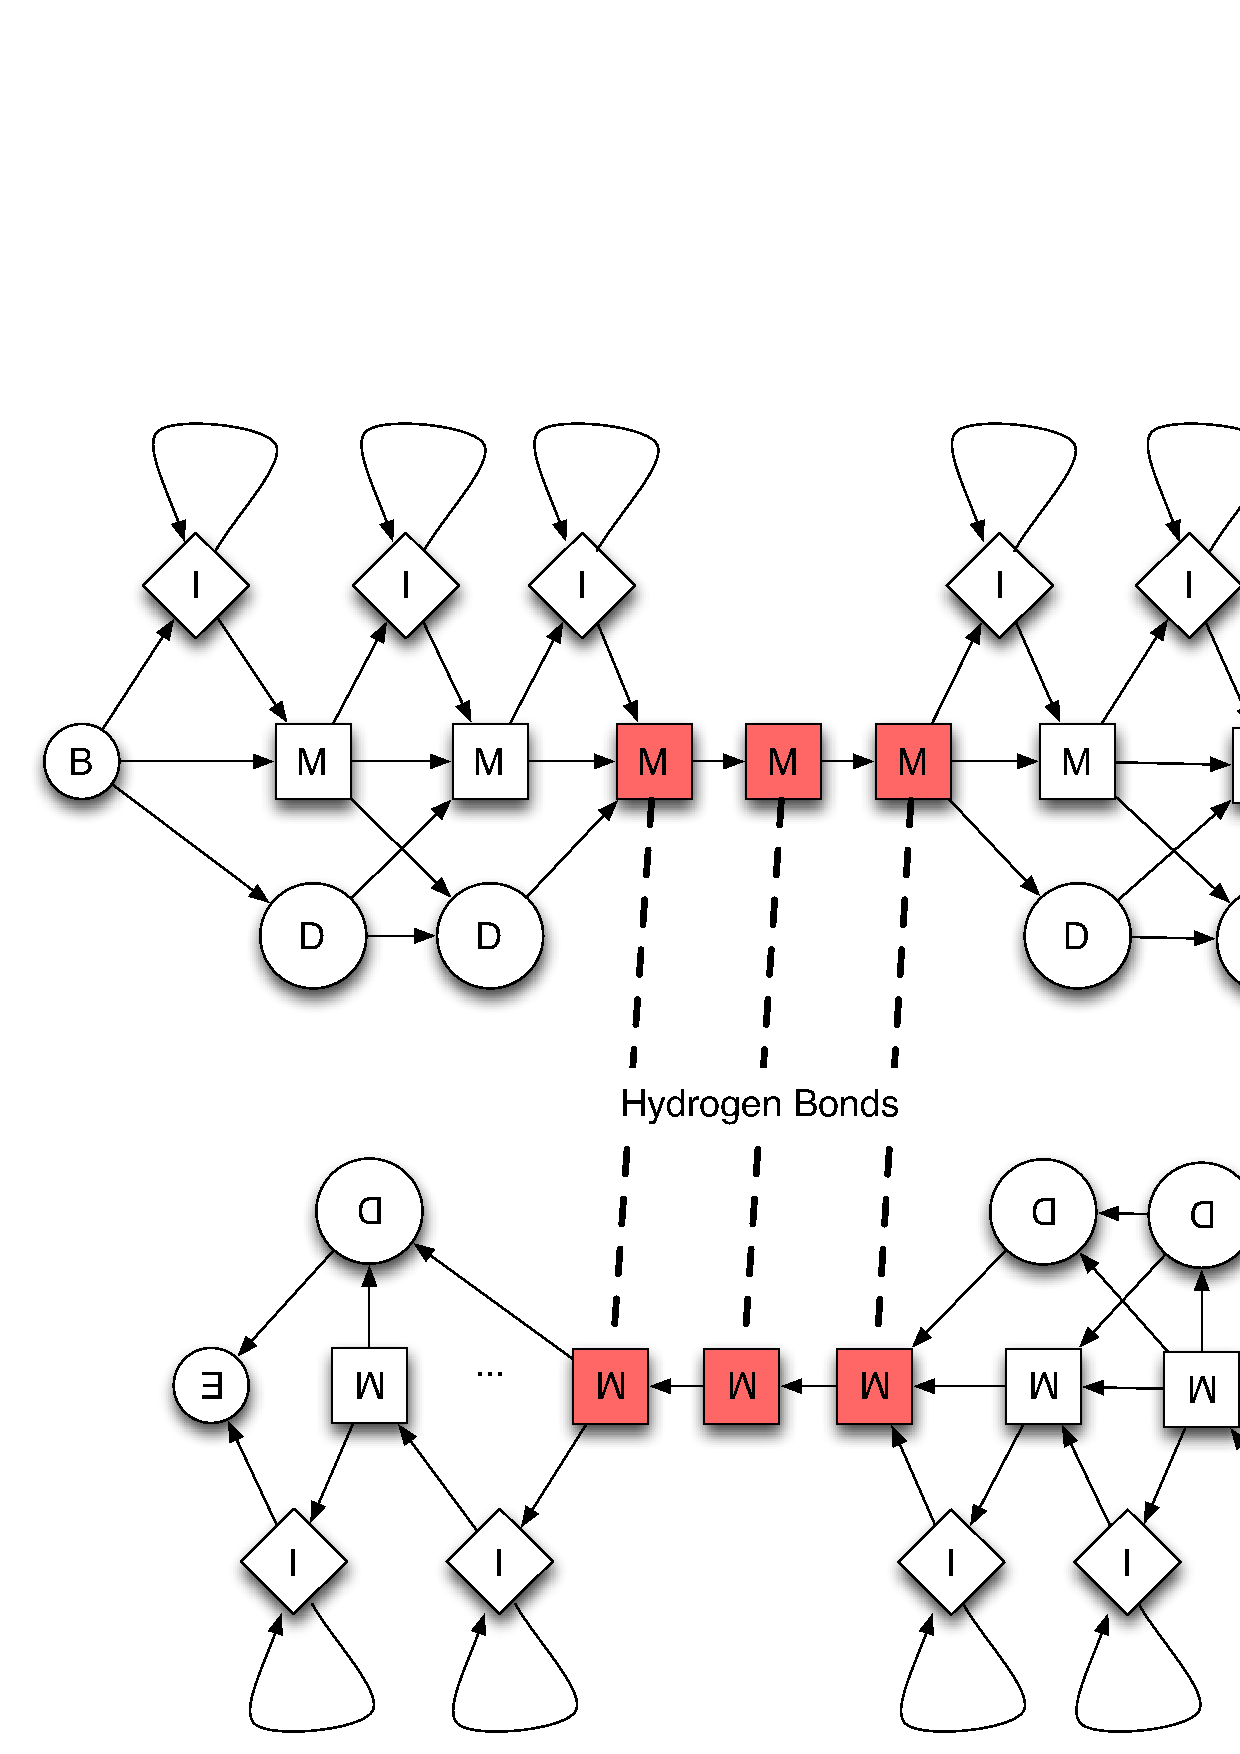
\includegraphics[width=11cm]{mrf_interleave_diagram.pdf}} 
\else
\centerline{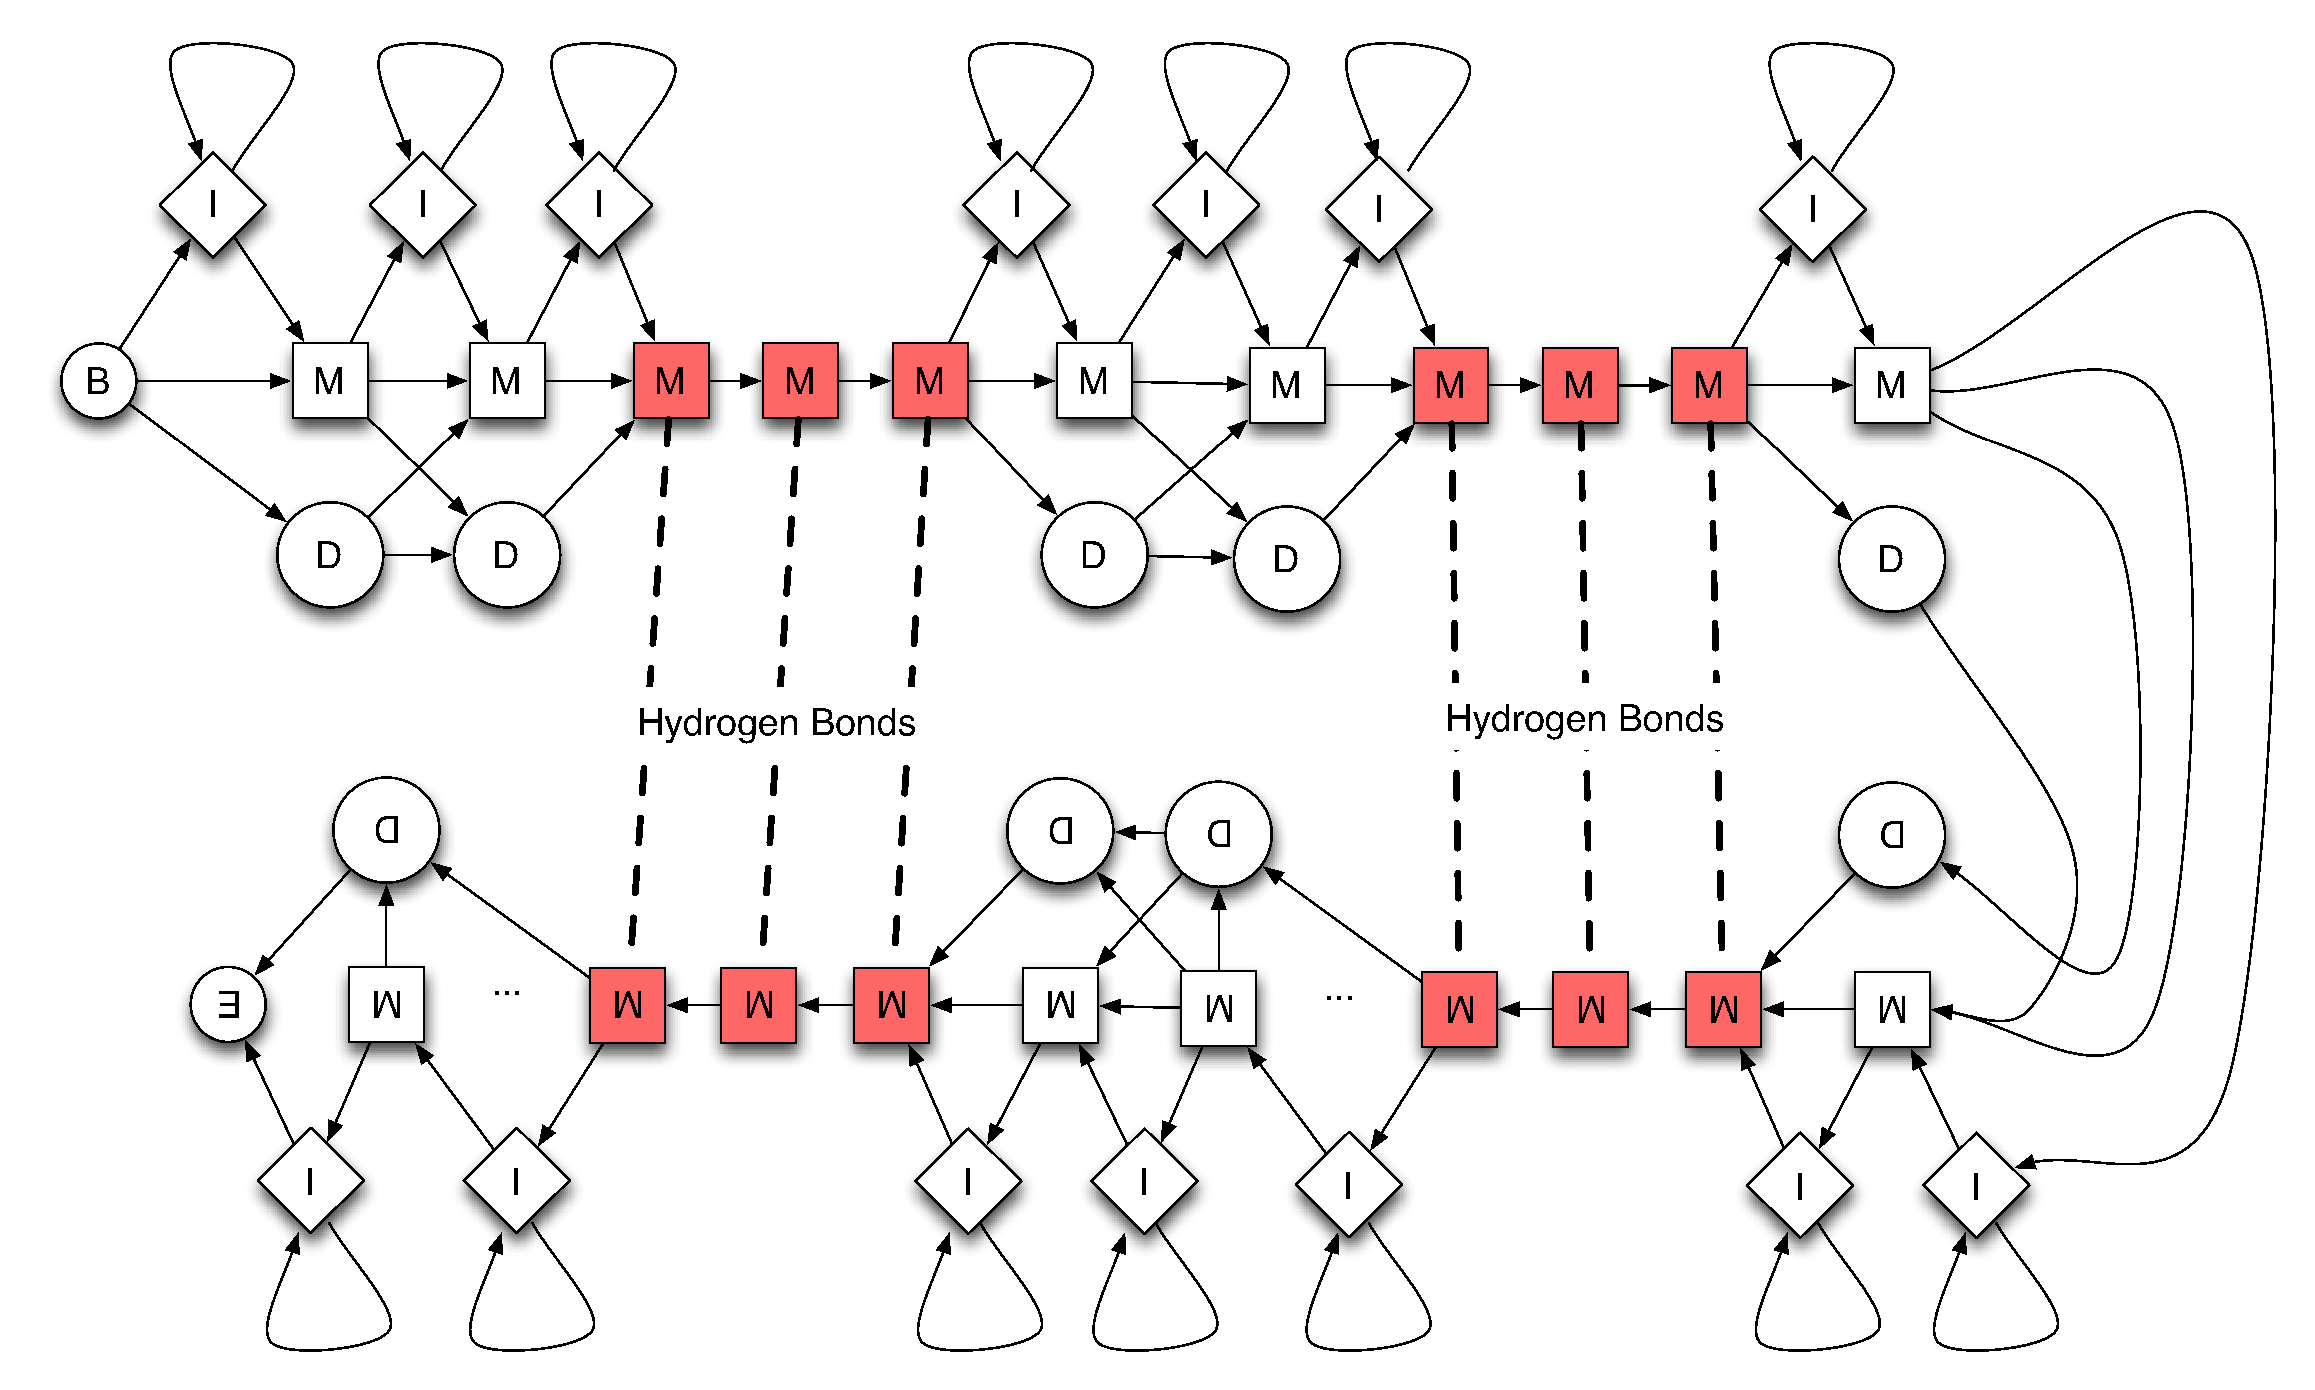
\includegraphics[width=11cm]{mrf_interleave_diagram.eps}} 
\fi
Each shaded node represents a beta-strand position.\\
Nodes connected by dashed edges are hydrogen-bonded.

\smallskip

\caption{A Markov random field with two beta-strand pairs}
\figlabel{mrf} 
\end{figure}



The new equations are accompanied by a new model.
Within a beta strand, amino acids are not inserted or deleted, so~a
bonded pair of beta strands is modeled by 
 a pair of sequences of match states.
Between beta strands, the model is structured as before.
The~combined model, an~example of which is shown in \figref{mrf}, is called a
\textit{Markov random~field}. 


%
% N.B. very tight paragraph...
%
MRFy treats the beta 
strands in the model
 as ``beads'' which can slide along the query sequence.
A~positioning of the beta strands is called
 a \emph{placement}.
A~placement's likelihood is computed
based on frequencies of amino-acid pairs observed in 
hydrogen-bonded beta strands~\cite{Cowen:2002p588}.
Given a placement, the maximum likelihood of the rest of
the query sequence, between and around beta strands,
is computed quickly and exactly 
using Viterbi's algorithm.
\iffalse
This likelihood is \emph{conditioned} on the placement.
\else
The exact result is a probability that is
\emph{conditioned} on the placement.
\fi

MRFy searches for likely placements stochastically.
\mrfy\ implements
random hill
climbing, simulated  
annealing, multistart simulated annealing, and a genetic algorithm.
These algorithms share much code, and \mrfy\ implements them using
higher-order functions, 
existentially 
quantified types, and lazy evaluation.




We~describe \mrfy's search abstractly: \mrfy\ computes a sequence
of \emph{points} in a search space.
The type of point is existentially quantified, but it is typically
a single placement or perhaps a population of placements. 
Each point also has a \texttt{Score}; \mrfy\ looks for points with
good scores.





Ideally, MRFy would use the now-classic, lazy, modular
technique advocated by \citet{hughes:why}, in which one function
computes an infinite sequence of points, and another function
uses a finite prefix to decide on an approximation.
But because MRFy's search is stochastic, 
making MRFy's search modular is not so easy.

To illustrate the difficulties, we~discuss our simplest search:
random hill climbing.
%The space of beta-strand placements has no notion of slope or
%gradient,
From any given point in the search space, this search moves a random
distance in a random 
direction.
If~the move leads to a better point, 
we call it \emph{useful};
otherwise it is \emph{useless}.
\smallverbatiminput{utility}
(We~also use \texttt{Useful} and \texttt{Useless} to tag \emph{points}.)
With luck, an~infinite sequence of useful moves converges
at a local optimum.

\mrfy's search path follows only useful moves;
if a move is useless, 
\mrfy\ abandons it and moves again (in a new random direction) from the
previous point.
The~search is depicted graphically in \figref{search-moves}.
Solid lines represent useful moves; dashed lines represent
useless moves.
The~points are laid out vertically in the order in which they are
discovered;
as you move downward, time increases.
Horizontally, we~have organized the points into five columns; 
the bottom point in each column is useful, and
any points above it in the same column are useless.


\begin{figure}
\tabcolsep=0.5cm
\centerline{%
\begin{tabular}{cc}
\loadpdf[scale=0.35]{search-figs/search-graph1}&
\loadpdf[scale=0.35]{search-figs/search-graph5}\\
\begin{minipage}{4cm}
\caption{Stochastic search with useful and useless moves}%
\figlabel{search-moves}
\end{minipage}%
&
\begin{minipage}{4cm}
\caption{Filtering out useless moves could cause nontermination}%
\figlabel{filtered-search-moves}
\end{minipage}\\
\end{tabular}%
}
\end{figure}

If~\mrfy\ could apply Hughes's technique, it~would search by composing
a~\emph{generator} 
that produces an infinite sequence of moves, 
a~\emph{filter} that selects the useful moves, and 
a~\emph{test} function that enumerates finitely many useful moves
and returns the final destination.
But~a~generator may produce an infinite sequence of useless moves.
For example, if \mrfy\ should stumble upon a global optimum, every move from
that point would be useless.
Given an infinite sequence of useless inputs, a~filter would not
produce any values, and the search would diverge.
This situation is depicted graphically in
\figref{filtered-search-moves}:
on the left-hand side, 
the first move is useless, the second move is useful, and all
subsequent moves are useless.
Filtering out useless moves would produce the sequence shown on the
right-hand side, which contains two points followed by a divergent
computation. 

We~avoid the possibility of divergence by combining ``generate and
filter'' into a 
single abstraction, which has type \mono{SearchGen pt r}.
Type variable~\texttt{pt} is a point in the search
space, and \texttt{r} is a
random-number generator.
\mono{Rand~r} is a lazy monad of stochastic computations:
\smallverbatiminput{gen.tex}
The monadic computation \texttt{pt0} randomly selects a starting point
for search;
\texttt{nextPt} produces a new point from
an existing point.
Because scoring can be expensive, both \texttt{pt0}
and \texttt{nextPt} use \emph{scored} points, and they can
reuse scores from previous points.

To tell if a point returned by \texttt{nextPt} is useful, we call
 the \texttt{utility} function,
which scrutinizes a move represented as follows:
\smallverbatiminput{move}
The decision about utility uses not only a source of randomness but
also the \emph{cumulative cost} of the point, which we define to be
the number of points explored previously.
The~cumulative cost of the current point is also the age of the
search,
and
in~simulated annealing, for example, as the cumulative cost increases,
the \texttt{utility} function becomes less likely to accept a move
that worsens the score.
To~attach a cumulative cost to a point, we use type \texttt{CCosted}:
\smallverbatiminput{aged}

Using these pieces, function \texttt{everyPt} produces an infinite
sequence containing a mix of useful and useless points.
Each useful point is tagged with cumulative cost and its score:
\smallfuzzverbatiminput{6pt}{everygen}
Both \texttt{nextPt} and \texttt{utility} are monadic, but 
we can still exploit laziness:
from its starting point, \texttt{everyPt} produces an infinite list of
randomly chosen successor points, then calls \texttt{costedUtility} to
tag each one with a cumulative cost and a utility.
Because we want to compose monadic computations in the same order we
compose ordinary functions, 
our code uses the monadic composition
operator~\texttt{=<<}, which is the bind operator with its arguments
swapped.


If \mrfy\ used Hughes's classic model of lazy search,
we~might expect to see an infinite sequence of points obtained by
applying \texttt{nextPt} to many points in succession, as~done by
the Prelude function \texttt{iterate}.
But~that's not how \mrfy\ works;
instead, 
the~infinite list \texttt{successors}
is computed by applying \texttt{nextPt} to
the \emph{single} initial point \texttt{startPt}, 
repeated infinitely many times.
Each repetition uses a
distinct source of random variation.

To~understand the structure of
 \mrfy's more complex search, it~may help to
relate the code to \figref{search-moves}.
Please assume that \texttt{startPt} is the point in the upper left
corner of \figref{search-moves}.
Then the first part of the \texttt{successors} list appears in the
next column:
the~first four elements are \texttt{useless};
the next element, which is the first useful point, is~\texttt{pt};
and~the remaining elements, which are never evaluated and are not
shown in the figure,
match the
underscore.
The first useful point \texttt{pt} is located by \mono{span~isUseless}.
After the search reaches~\texttt{pt},
we~start the search anew with a recursive 
call to \mono{everyPt~sg}, 
passing~\texttt{pt}.
%
The~most informative part of \texttt{everyPt} is last expression of
the \texttt{do} block,
which shows that the result begins with a useful point,
is followed by a (possibly infinite, possibly empty) list of useless
points, and then continues with the results of a recursive call
to \texttt{everyPt}. 





\mrfy's search may explore an arbitrary number of infinite
lists of points, each reached using a different source of randomness.
We~suppose this search space could be represented by a single
value of type \mbox{\mono{Rand r [[Scored pt]]}}, but when writing
client code, we~found it much easier to think about the
representation we actually use in the
\texttt{SearchGen} record:
the~monadic value
\texttt{pt0} together with the function \texttt{nextPt}.



%%\begingroup\parskip=0.9\parskip
%% \makeatletter\@sectionaboveskip=0.9\@sectionaboveskip\makeatother

\vfilbreak{2.5\baselineskip}

The rest of the search uses Hughes's
classic composition of generator  and test function.
\smallverbatiminput{search}
The \texttt{test} function has type \mono{SearchStop~pt}:
\smallverbatiminput{stop}
Type \mono{History~pt} retains only the useful points.
(Internally, \mrfy\ needs only the \emph{final} useful point,
but because we want to study how different search algorithms behave,
we~keep all the useful points.)

The definition of \texttt{SearchStop} reveals two forms of
non-modularity which are inherent in \mrfy's search algorithm.
First, we need \texttt{Utility}, because if we omit the useless states,
search might not terminate.
Second, we need \texttt{CCosted}, because some of our test functions
decide to terminate based either on the cumulative cost of the most
recent point or on the difference between costs of successive useful points.

Despite these non-modular aspects, the search
interface provides ample scope for
experiments.
Random hill climbing took 50~lines of code and one~day to
implement.  
Simulated annealing required only a new
\texttt{utility} function, which took 15~lines of code and half an hour to implement.
(Hill climbing accepts a point if and only if it scores better than its
predecessor;
simulated annealing may accept a point that scores worse.)
Our genetic algorithm uses very similar
functions, except for \texttt{nextPt}:
recombination of parent
placements took forty lines of code
and a full day to implement.

We're not entirely happy with the way we're writing all the individual
functions.
In~particular, \texttt{SearchStop} functions aren't composable;
we~can't, for example, combine two functions to say that we'd like to
stop if scores aren't improving or if we've tried a thousand points,
whichever comes first.
Eventually, we'd like to have
combinator libraries for \texttt{SearchStop} and \texttt{nextPt}, at~least.

%%  Our \texttt{SearchStrategy} interface somewhat resembles an object-oriented
%%  style of programming.
%%  However, it is \textit{easier} to create a SearchStrategy
%%  in Haskell than using conventional object-oriented techniques, because
%%  all the functions in a SearchStrategy are partial applications of
%%  other functions.
%%  If we were using conventional object-oriented
%%  techniques, we would have to declare subclasses with instance
%%  variables and would have to write code to initialize objects of those
%%  subclasses. 


\subsection{Performance}

\seclabel{perf}
\seclabel{performance}

At each point in its search,
MRFy calls \verb+vee'+ several
 times.
Our~\verb+vee'+
function computes a \mbox{\mono{Scored [StateLabel]}}, that~is, 
an~optimal path and its score.
But at intermediate points in \mrfy's search,
\mrfy\ uses only the
score.
Even though Haskell evaluation is lazy, \verb+vee'+ 
still allocates thunks that could compute paths.
To~measure the relevant overhead,
we~cloned \verb+vee'+ and modified it to compute
only a score, with no path.
This change improved 
run time by nearly~50\%.
%%But when \texttt{search} finally decides on a placement, we need a
%%version of \verb+vee'+ that \emph{does} compute a path, so we can
%%extract the optimal parse for that placement.

Could we keep the improvement without 
maintaining two versions of \verb+vee'+?
In~Lisp or Ruby we would have used macros or metaprogramming,
but we were not confident of our ability to use Template Haskell.
Instead, we used higher-order functions.
As~shown in \secref{vee-prime},
\verb+vee'+ does not use primitive~\primcons\ but instead
uses an unknown function \texttt{cons}, which is
passed~in.
To~get a path, we pass in primitive~\primcons;
to~get just a score, we pass in
\verb+\_ _ -> []+.
This trick is simple and easy to implement, and it provides the same
speedup as the cloned and modified~code.
But~we worry that it may work only because of
undocumented properties of GHC's inliner, which may 
change.

Even with this trick,
MRFy's implementation of Viterbi's algorithm is much
slower than the C++ version in \mrfy's predecessor,
SMURF.
For example, on a microbenchmark that searches for a
structural motif of 343~nodes in a protein of 2000 amino acids
using only Viterbi's algorithm and no beta-strand information,
\mrfy\ takes 2.32~seconds and
SMURF takes 0.29~seconds.

But \mrfy's job is not to run Viterbi's algorithm on large models;
\mrfy's job is to detect homologies to structures for which both Viterbi's
algorithm and SMURF's more complex algorithm are unsuited.
\mrfy\ can solve problems that SMURF cannot.
For~example, we tried both programs on a complex, 12-stranded ``beta
sandwich'' 
model.
The~model contains 252~nodes,
97~of which appear in the 12~beta strands.
% The models between beta strands typically have at most 12~nodes.
% We used a query sequence of 237 amino acids, but each placement
% breaks the sequence into 13 pieces, each of which typically has at most
% 11~amino acids.
\mrfy\ computes an alignment in under a~minute,
but SMURF allocates
over 16GB of memory and does not terminate even after eight hours.


\begin{figure}%%%[h!]
\centerline{\loadpdf[]{speedup}}
\medskip
\caption{\mrfy's parallel speedup on an 8-bladed beta propeller}
\figlabel{speedup}
\end{figure}

We also benchmarked \mrfy\ using a model of an ``8-bladed beta propeller.''
The model has 343~nodes, of which 178 appear in 40~beta strands.
The segments between beta strands typically have at most 10~nodes.
We~used a query sequence of 592 amino acids, but each placement breaks
the sequence into 41~pieces, each of which typically has at most 20 amino
acids.
Because \mrfy\ can solve the models between the beta strands independently,
this benchmark has a lot of parallelism,
which Haskell made easy to exploit.
Using
\texttt{Control.Parallel}, parallelizing the computation was as easy
as  substituting
\texttt{parmap rseq} for \texttt{map}.
\figref{speedup} shows speedups when using from 
 1~to~48 of the cores 
on a 48-core, 2.3GHz AMD Opteron 6176 system.
Errors are estimated from 5~runs.
After about 12~cores, where \mrfy\ runs 6~times as fast as sequential
code, speedup rolls off.
By~running 4~instances of \mrfy\ in parallel on different searches,
we~hope to be able to use all 48~cores with about 50\%~efficiency.


%%  \begin{figure}[h!]
%%  \centerline{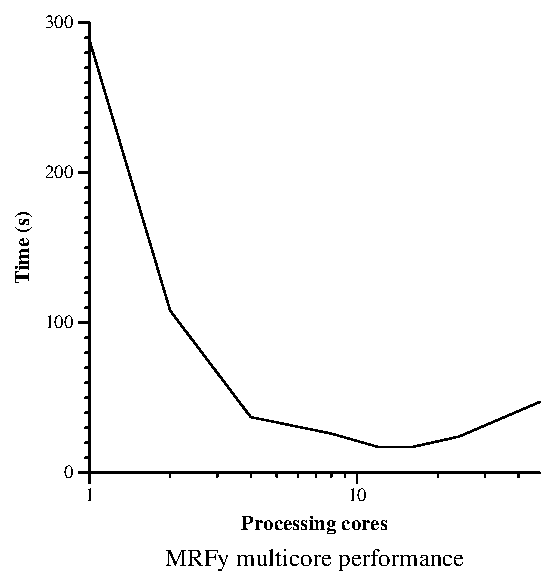
\includegraphics[width=6cm]{mrfy_multicore_log}}
%%  \caption{MRFy run-time performance with varying
%%  numbers of processing cores on a large protein}
%%  \label{multicore}
%%  \end{figure}


%%% Had we implemented the SMURF algorithm in Haskell, we believe that performance
%%% would be unacceptable.
%%% However, for the algorithm underlying MRFy, we are satisfied with the runtime
%%% performance of Haskell and GHC.
%
% Nonetheless, we expect that we can still improve MRFy's run-time performance
% with further profiling and tuning.  
% And we expect that if we cross the street, we will get to the other side.


\subsection{Improving \mrfy's sequential performance}

\seclabel{better-viterbi}
\seclabel{improving-viterbi}

Software for
computational-biology research doesn't have to be fast to be useful.
But~if \mrfy\ solves some problems 8~times slower then
SMURF, that's a poor showing for Haskell.
\mrfy\ spends 98\%\ of its time running Viterbi's algorithm, and
we~felt sure that with some love and attention, we could make it
more competitive with~C++.
But~before we could try to make \mrfy\ faster, we~had to make it simpler.

The code example for \verb+vee'+ on page~\pageref{code:vee-prime}
shows the computation of the general case of~$V^{\prime M}_j(i)$ from 
\figref{viterbi-transformed}.
But the full story is not as nice at one could hope for:
in~the code that accompanies our 2012 ICFP paper,
\verb+vee'+ has 25~cases overall.
Many of these cases exist because when we first wrote the code, we~did
not have enough insight into 
Haskell.
We~made some decisions that might have been more
appropriate to FORTRAN:
\begin{itemize}
\item
Recursive computations were done on smaller array indices, not smaller
models.
\item
Array indices 1, 0, and $-1$ were all used to indicate special
conditions.
\item
Senseless combinations of array indices and states were handled by
assigning each such combination the largest representable score, which
corresponds to the smallest representable probability.
\end{itemize}
%
%
To~simplify this code, we started thinking more like Haskell
programmers.
In~particular, we used types more effectively:
\begin{itemize}
\item
We~refactored the single, flat \texttt{Node} type from our ICFP paper
into the three state types you see on page~\pageref{code:model3-node}.
\item 
We introduced a \texttt{Model} type that consists of a special Begin
node containing a begin and an insertion state, an~unbounded sequence
of ordinary \texttt{Nodes}, and an end state.
And we represented the sequence as a list, not an array.
\item
We~observed that the main algorithm where \mrfy\ spends all its time
uses only match, insertion, and deletion states, so we removed the
\texttt{StateLabel} value constructors corresponding to begin and end
states, leaving only the three constructors shown on
page~\pageref{code:state-label}. 
(We~moved the begin and end labels to another type, which is used only
to prettyprint models.) 
\end{itemize}
The immediate effect of these changes was to reduce case analysis along
two dimensions:
instead of five state labels, we got three;
and instead of three special array indices, we got just one special
list (the empty list).

\begin{figure}
\noindent\hspace*{1.5cm}\begin{minipage}{11cm}
\smallverbatiminput{list-viterbi}
\smallskip
\end{minipage}

\caption{Sketch of Viterbi's algorithm, using lists}
\figlabel{list-viterbi}
\end{figure}

To~reduce case analysis even more, we~abstracted over state labels.
\figref{list-viterbi} sketches the structure of the algorithm.
\figref{viterbi-hov4} is the first example in this paper that
shows \emph{all} the cases for~\verb+vee'+.
It~reduces the original 25~cases to just~4.
We~show only a sketch because we didn't use this version in
production.
The difficulty was in memoizing a \verb+vee'+ that takes lists as
arguments. 
We~built and tested specialized memo combinators that work
with list prefixes, but 
we~were never confident that the resulting code would be simple,
correct, and efficient.
Instead, we~used insights from the list-based code to create a new
array-based version:
\begin{itemize}
\item
We~kept the abstraction over \texttt{stateHat}, which we explain
below.
\item
We~got the idea that if we have to compute with integers, we~want
$i$ to \emph{count} the number
of amino acids in the sequence~\texttt{aas}, 
but we want $j$ to \emph{index} into an array of nodes.
\item
From
\figref{list-viterbi}'s \texttt{next} function, we~got the idea that
Viterbi's algorithm 
computes a minimum edit 
distance.
This idea didn't affect the code directly, but as we experimented with
new variations, it~helped us keep track of the big picture.
\end{itemize}
Armed with these ideas, we~turned back to computing with arrays and
integers. 


\def\p#1{\mathit{p#1}}
\begin{figure}
\def\vsum#1#2{#1+#2}
\[
\begin{array}{r@{}c@{}l}
\multicolumn3{c}{
  V_{j}^{\prime \hat s}(i) = e^{\prime}_{\hat s_{j}}(x_{i}) 
    + \min\limits_s \big\{
         \vsum{V_{\mathit{\p j}}^{\prime s}(\p i)} 
     {a^{\prime}_{s_{\p j} \,\hat s_j}}, 
      \mbox{ where $s$ can precede $\hat s$ and $\p i = \widetilde{\p i}\; s$}  \big\}
}
\\[10pt]
\mbox{where }\widetilde{\p i}\; s&{} = {}& 
  \left\{ \begin{array}{l}
          i \mbox{, if $s=D$}\\
          i-1 \mbox{, otherwise}\\
          \end{array}
  \right.
\\[10pt]
\p j &{} = {}& 
  \left\{ \begin{array}{l}
          j \mbox{, if $\hat s=I$}\\
          j-1 \mbox{, otherwise}\\
          \end{array}
  \right.
\\
\end{array}
\]

\caption{Viterbi's equations, abstracted over state~$\hat s$, 
defining $e^{\prime}_{D_j}(x) = 0$}
\figlabel{viterbi-abstracted}
\end{figure}

\figref{list-viterbi} shows a sketch in which the state
label \texttt{stateHat} is abstract.
We~kept that abstraction, and
we~now turn your attention to how it works.
In~Viterbi's equations,
$V'$ is indexed by a residue count~$i$,
a~node index~$j$,
and
a state label $M$, $I$, or~$D$.
Each state uses a slightly different equation, but it is possible to
combine them.
\figref{viterbi-abstracted} shows a single equation which, when
state $\hat s$ is specialized to state $M$, $I$, or~$D$, becomes one of the
original three equations from \figref{viterbi-transformed}.
The figure adds the cost of emitting an amino acid at state~$\hat s$
to the lowest of the costs of the paths entering~$\hat s$ from predecessor
state~$s$.
Index~$\p j$ is the index of the node containing the predecessor
state.
Integer $\p i$~counts the number of amino acids emitted before~$\hat
s$ and so is the index of the amino acid, if~any, to be
emitted at state~$\hat s$.

To~implement \figref{viterbi-abstracted}, we~define several
auxiliary functions.
The~set of states that can precede~$\hat s$
is \mono{preceders~$\hat s$}; $\p i$~and~$\p j$ are computed using
function \texttt{predUnless}:
\smallverbatiminput{v4aux}
We~also use \texttt{newtype} to define 
a value constructor~\texttt{RC} for a residue count~$i$
and
a value constructor~\texttt{NI} for a node index~$j$.
Given these tools, we~built the abstract, array-based version of
Viterbi's algorithm 
shown in \figref{viterbi-hov4}.
Auxiliary functions \texttt{node} and \texttt{residue} do array
indexing, and functions \texttt{transmission} and \texttt{emission}
are variations of the functions \texttt{aScore} and \texttt{eScore}
mentioned in \secref{aScore}.


\begin{figure}
\noindent\hspace*{1.0cm}\begin{minipage}{11cm}
\smallverbatiminput{hov4}
\smallskip
\end{minipage}

\caption{Viterbi's algorithm abstracted over~$\hat s$, with signatures
of auxiliary functions}
\figlabel{viterbi-hov4}
\end{figure}


The version of \verb+vee'+ shown in  \figref{viterbi-hov4} is abstract
in another way: the type of the result is an unknown type~\texttt{a}.
Type~\texttt{a} represents a tree-node in an abstract ``cost~tree;''
we~instantiate it as a score, as a \mono{Scored~[StateLabel]},
and as an explicit tree used to visualize and debug the computation.
Values of type~\texttt{a} are built using three functions that are
passed as parameters:
\smallverbatiminput{hosigs}
The \texttt{internal} function must treat an empty list of edges as an
unreachable tree-node; for~example, if \texttt{a} is instantiated
to \texttt{Score}, then \mono{internal~[]} must produce an infinite
score (corresponding to zero probability).

The~three base cases in \figref{viterbi-hov4} are not exactly the same
as the base cases in \figref{list-viterbi}.
In~\figref{viterbi-hov4}, the base cases
handle the three states that can
follow the begin state.
In~our legacy file format, and also in our code, the begin state is
identified with the match state in node~$j=0$.
But although it is
identified with a match state, the begin state does not behave like a
match state: it~does not emit a residue.
Therefore the three states that can follow it can be entered only when the
count of residues emitted is~$i=0$.

Using the code in \figref{viterbi-hov4}, plus the auxiliary functions
shown above, the implementation of Viterbi's algorithm is just
25~lines of code, of which 2~lines are type signatures.
That's four times smaller than our original code.
But~while we've gained something, we've also lost something---it's not
at all obvious that the code in \figref{viterbi-hov4}  implements
Viterbi's equations.

Our~original goal was to make Viterbi's algorithm faster.
To~measure its speed, we~created a benchmark that runs only Viterbi's
algorithm, but on inputs that mimic the way \mrfy\ is intended to be used.
The benchmark contains 56 protein sequences and 9 hidden Markov
models.
The query sequences are taken from the from the deep-sea 
bacterium \emph{Thermotoga maritima}, and they 
range in length from 80 to 1200 residues.
The models are each built from a multiple-structure alignment of the
proteins in 
a $\beta$-structural protein superfamily.
To~run the benchmark, we read in the query sequences and the models,
and we compute the score of the best alignment of each sequence
against each model.
Using GHC~7.4 on~an Intel Ivy Bridge Core i5-3570 CPU clocked at
3.4GHz, this benchmark takes about 45~seconds to~run.
\mrfy\ spends most of its time garbage collecting and 99\%\ of the
remaining time running Viterbi's algorithm.
Time~spent in I/O and parsing is only about 0.2\%~of the
total.

Using this benchmark, the new code wasn't much different from the old
code---just about 3\%~slower.
But it 
was a good starting point for experiments.
We~tried myriad variations, 
the best of which involved two transformations:
\begin{itemize}
\item
We~abstracted the call to \texttt{internal} over the state~$\hat s$,
the list of preceding states, and functions that
compute \texttt{pi}~and~\texttt{pj}.
\item
We~added a fourth case to \verb+vee'+, which handles the match
state in node~1 when the residue count is nonzero.
\end{itemize}
For reasons we don't understand, GHC specializes the resulting code
very effectively, leading to 30\%~faster performance on our
benchmark.
The~result is 26\%~faster than our original code.

One of the variations that didn't help, surprisingly, was
to follow
\citet{tibell:high-performance} and use GHC's UNPACK pragma on scalar
values---in our case, scores.
Although using the UNPACK pragma made our original code 7\%~faster, it
makes the new
code 9\%~slower.

To~develop a more detailed understanding of performance, we~turned
to GHC's profiler.
We ran Viterbi's algorithm on a single query sequence
of 592~residues, against a
model of 343~nodes.
The~profiler told us that a lot of time was spent in memory
management, and that \mrfy\ allocated a total of 531MB.
\mrfy's main data structure is the memo table used for \verb+vee''+, 
which has one entry for each combination of
$\hat s$, $j$, and~$i$.
In~this run, that's 610,197 entries.
We~expected \mrfy\ to use an amount of memory proportional to the
size of the memo table.
But the constant of proportionality is 7.85KB, which seems excessive.
We~hoped that the detailed profile would explain, but it
contained some information we
understood and some we didn't.
\begin{itemize}
\item
The most easily understood source of allocation
is the function \verb+vee''+, which is charged with
allocating about 66MB.
What \verb+vee''+ does is call memo combinators,
so the 66MB might be the memo table.
To~evaluate this hypothesis, we~estimated the amount of memory that
might be consumed by a memo-table entry.

Once evaluated, a memo-table entry will contain a pointer to a
double-precision floating point number allocated on the heap.
The~pointer itself should occupy a word, and representing a
boxed \texttt{Double} on the heap might
require three 32-bit words.

Before it is evaluated, a memo-table entry should contain a thunk
involving the parameters $\hat s$, $j$, and~$i$.
Such 
a~thunk might be a bit like a four-element
list, taking perhaps 12~words for the cons cells and another 8~words
for  values.

By this estimate we could expect
24~words per entry times 4~bytes per word, which would be 96B per
entry and a total of about 59MB.
Because the actual memo table involves arrays of arrays of arrays,
we~won't quibble about a discrepancy of~10\%; 
our estimate of the memory taken by the memo table seems accurate
enough, and we~can think of nothing we can do to improve it.
\item
Another source of allocation---one that surprised us---is the 
computation of \texttt{score}, which is the let-bound sum of transition 
and emission scores in \figref{viterbi-hov4}.
This binding is charged with allocating 45MB total, or about
4.5~words for each transition in the computation tree.
The~\texttt{edge} function is strict in the first argument, which
is \texttt{score}, and we don't know why the computation is allocating.
As~an experiment, we tried to make
the sum strict by using a bang pattern in 
``\mono{let~!score = }\ldots''
While this change eliminated \texttt{score} as a source of allocation,
the allocations moved somewhere else, because the total number of
bytes allocated increased very slightly, by just 12B.
\item
On~this much smaller input, 16\%\ of the allocation is done by the
code that reads and parses the model and the query sequence.
We~don't care about improving that part.
\item
The single most expensive part of the program
is the function \verb+vee'+ itself, which
allocates 258MB---half of all memory allocated.
We~have no idea what is happening.
A~graphical heap profile shows a large amount of memory initially
charged to \verb+vee''+ (the memo table), which then shrinks
gradually, presumably as large thunks are replaced with smaller
scores.
The~amount of memory charged to \verb+vee'+
increases roughly linearly with time, 
so~perhaps we have a space leak, but even given the various profiling
tools available, we~were not able to find~it.

To~try to eliminate the unwanted allocations,
we~explored many variations on the code, of~which the most ambitious (and
most tedious) was to desugar the list comprehension by~hand and to
replace standard list operations with counterparts that participate
in stream fusion \cite{coutts:fusion}.
Nothing~helped.
\end{itemize}
In~desperation, we~tried to diagnose our problems by reading 
Core output from~GHC.
We~were guided by Don Stewart's invaluable blog posts,
and we also used his \texttt{ghc-core} tool, 
but it wasn't enough.
Even though one of us has worked on several optimizing compilers, 
we~just don't have enough experience to use GHC Core to diagnose
allocation problems in a 25-line function.





%%\begin{verbatim}
%%### 2013-05-27 01:23   Running med(vpasses=1): icfp-branch mrfy nr-jfp
%%icfp-branch faab8dc       54.07s    i686  GHC 7.4.1  Core i5-3570 @ 3.40GHz
%%mrfy d5604bc*             44.90s    i686  GHC 7.4.1  Core i5-3570 @ 3.40GHz
%%nr-jfp 00ef54e*           47.59s    i686  GHC 7.4.1  Core i5-3570 @ 3.40GHz
%%\end{verbatim}




%%\smallverbatiminput{hov-prevs}

Our efforts to improve \mrfy's sequential
performance concluded unhappily.
Although we made Viterbi's algorithm a lot simpler and somewhat
faster, it~is still nowhere near competetive with~C++.
The measurements using SMURF are depressing enough, but because we were
not entirely sure what SMURF was doing, we wrote a fresh,
``cleanroom'' implementation of Viterbi's algorithm in~C, using
forward dynamic programming.
To~avoid writing a parser, we extended \mrfy\ with a function that reads a
model and a query sequence and emits a C~file containing that model
and query as initialized data.
On~a synthetic benchmark involving all pairs of three models and three
query sequences, our new C~code runs about 45~times faster than \mrfy.
Ironically, we've~had a lot of trouble getting the C~code right, but it
allocates only one double-precision floating-point number for each
entry in the memo table.
Haskell allocates about 30~times more.

It's depressing to think that a language with a mature, optimizing,
native-code compiler might not be usable for performance-critical
work, but the difficulty of diagnosing allocation problems is a real
obstacle.
We~were lucky that we could get new results
even though our core algorithm is 45~times slower than the
same algorithm written in~C.
You~might not be so lucky.



\subsection{Debugging and testing: awkward at first, but then  less awkward}

\seclabel{awkward-profiling}

Because we got lucky, the difficulty of understanding Haskell's
allocation behavior didn't present the obstacle it might have.
But we did encounter other obstacles that prevented functional
programming from working as well as we would have liked.
The~most significant such obstacles were in debugging and testing.

We~started \mrfy's development using GHC~7.0, and
we had a hard time diagnosing run-time errors.
Run-time errors were something we expected to deal with;
our~group's legacy file
format is poorly documented, and code that reads it usually contains
faults. 
(When beta
strands overlap and are doubly paired, even the invariants of the
format are unclear.)
But~even though we expected run-time errors, we~found them hard to diagnose.
Our code became littered with
calls to
\texttt{trace}, 
even when we relegated \texttt{trace} to wrapper functions.
We~didn't know about the backtrace feature of GHC's profiler,
and even after we learned about it, it didn't help:
that profiler could be used only on very small test cases,
which didn't always trigger the errors.

The problems with run-time errors and profiling were all fixed in
February~2012, when GHC~7.4 was released.
By~that time our code had matured, and run-time errors were no longer
a significant issue, but occasionally we still appreciate the ability 
to get a stack trace on error.

While we were wrestling with run-time errors, we~also tried to use
GHCi's debugger, but it was too limited:
in~GHCi, our \texttt{vee'} function
is too slow to be runnable on nontrivial
inputs.
Moreover,  GHCi's debugger can set breakpoints only at top-level functions
or at specific column/line positions, which made debugging the memoized
\texttt{vee''} function impractical.

Our difficulties with debugging led to internal disagreements.
The~junior members of our team wanted to apply the debugging
skills they had honed through years of imperative programming.
But these skills did not transfer well to Haskell.
The senior member of the team kept repeating that a proper approach to
debugging Haskell code should involve QuickCheck.
But mere exhortation was unhelpful.

\seclabel{awkward-quickcheck}

Only the senior member of our team was able to use
QuickCheck easily.
In~retrospect, we~have identified some obstacles that prevented the
junior people from using
QuickCheck.
\begin{itemize}
\item
The examples and tutorials we found focused 
on writing and testing properties using data types that
already implemented class \texttt{Arbitrary}.
We~didn't understand the \texttt{Arbitrary} class very well, 
perhaps because the overloaded \texttt{arbitrary} value is not a
function.
(For programmers accustomed to object-oriented dispatch
on \emph{arguments}, it is hard to grasp how Haskell's type-class
system can find the proper version
of \texttt{arbitrary} using only the type of a \emph{value}.)
\item
Our difficulties were compounded by a weak understanding of monads.
We~were too baffled by QuickCheck's \texttt{Gen} monad to grasp its
importance.
\item
We~continually overlooked the critical role of \emph{shrinking}.
As~a result, on the one or two occasions we did 
use QuickCheck, the counterexamples were too large to be
informative. 
To~be fair to ourselves, the \texttt{shrink} method is barely
mentioned in the original 
paper on QuickCheck \cite{claessen:quickcheck};
it~shows up under another name and is described as~an improvement made
by Andy Gill. 
\end{itemize}
Because of these obstacles, 
we wrote thousands of lines of code without ever defining an instance
of \texttt{Arbitrary} and therefore
without looking hard at QuickCheck.
After the fact, we were overwhelmed by the work
involved in writing and testing instances
of
\texttt{Arbitrary}.
The work got done only when the whole team pitched in to
meet deadlines for ICFP~2012.

After ICFP, 
QuickCheck played a central role in further developments.
Most important was the testing of the variations on Viterbi's
algorithm described in \secref{better-viterbi}.
We~used QuickCheck not only to shrink sequences of nodes and of amino
acids, but also to shrink the number of nonzero transmission and
emission probabilities in the models.
We~were able to confirm that each new implementation computed the same
paths with the same score as our original implementation.
Almost all counterexamples were shrunk to include just two nodes 
(the smallest model supported by our original implementation)
and two or three residues.
Moreover, the models contained just a handful of nonzero
probabilities.
QuickCheck played an invaluable role in helping us get edge cases
right, and in confirming that most of the cases in the original code
could be eliminated.



%%  At~that point, we were quickly about to write QuickCheck
%%  specifications for several properties of the Viterbi algorithm:
%%  \begin{itemize}
%%  \item
%%  The total number of \verb+Mat+ and \verb+Ins+ states returned equals
%%  the number of amino acids in the query sequence.
%%  \item
%%  The total number of matches, and deletions returned equals the
%%  number of nodes in the hidden Markov model,
%%  \emph{except} that an initial sequence of
%%  of~\verb+Ins+ states counts as a single node,
%%  due to an odd property of the HMMER file format (namely, the zeroth
%%  node has no delete state and a non-emitting match state which
%%  is always occupied, but a normal insert state).
%%  \item
%%  The sequence returned satisfies the Plan7 invariant, that is, states
%%  \verb+Ins+ and \verb+Del+ are never adjacent.
%%  \end{itemize}
%%  \textbf{These properties need to be followed by more ambitious
%%  properties},


 
 
\section{Our previous experience compared}
\seclabel{comparo}

Our Haskell code for hidden Markov models and Viterbi's algorithm
solves the same problems as existing C++~code.
Other researchers using Haskell may also have to reimplement code,
but
in computational biology, reimplementing existing algorithms is unremarkable.
For~example, both SMURF and HMMER also contain new implementations of
hidden Markov models and Viterbi's algorithm.

When performance has mattered, members of our group, like other
computational biologists, have used~C++.
To~compare our Haskell experience with our C++ experience,
we discuss three tools:
\begin{itemize}
\item
Matt~\cite{Menke:2008wu} is used to create alignments like that shown
in \figref{alignment}.
It~comprises about 12,000 lines of~C++.
The only external tools or libraries it uses are \texttt{zlib}
and \texttt{OpenMP}, and its initial development took two years.
\item
SMURF
\cite{Menke:2010ti} is used to detect homologous proteins in the presence
of paired beta strands.
It~comprises about 9,000 lines of~C++, of which about 1,000~lines are
shared with~Matt.
It~uses no external tools or libraries, and
its initial development took a year and a half.
It uses multidimensional dynamic programming to exactly compute the alignments
for which MRFy relies on stochastic search.
As a result, in the presence of complex beta-strand topologies, SMURF is
computationally intractable.
\item
MRFy is used to detect homologous proteins in the presence of paired
beta strands; it effectively supplants SMURF.
It~comprises about 2,500 lines of~Haskell, about 500 of which are devoted
to tests, QuickCheck properties, and generators.
Neither Matt nor SMURF includes test code.
MRFy~uses several external tools and libraries, of which the most
notable are Parsec, the BioHaskell bioinformatics library, and
the libraries \path{Data.MemoCombinators}, \path{Control.Parallel},
and \path{Data.Vector}.
\mrfy's initial development took about three months.
%%%% \remark{Others were mostly full-time work, but no need to distinguish.}
\end{itemize}
Like much research software, all three tools were written
 in~haste.
And all three have later been modified.

% \ifpagetuning\enlargethispage{\baselineskip}\fi


We~modified Matt to use information about sequences as well as structure.
The modification added 2,000 lines of code, and it calls
external sequence aligners that we did not write.
We~thought the modification would take three months, 
but it took most of a~year.
Matt uses such
data structures as mutable oct-trees, vectors, and arrays.
It~uses clever pointer arithmetic.
The mutable data structures were difficult to 
repurpose, and the pointer arithmetic was \emph{too} clever: 
nearly every change resulted in new~segfaults.

We~had hoped to extend Matt further, with support for partial alignments,
which we~expected to require only 
a cosmetic manipulation of the 
output.
But
this feature wound up
requiring deep information about Matt's data structures,
and we had to give~up.
We~believe we could write an equivalent tool in~Haskell
% with most of Matt's performance, % HA!
in at most nine months.

Our most painful experience was adding ``simulated evolution''
to~SMURF \cite{Daniels:2012}. 
Although simulated evolution represents a relatively minor
enhancement,
just understanding the existing code took several months.

We~built MRFy quickly, and we expected that
higher-order functions would make MRFy easy to extend.
Each new addition to MRFy's stochastic search took at most a day
to implement.
However, the next extension we wished to make
was based on
Richard Senington's model of \emph{local
search} \cite{senington:hybrid}, 
which does not fit our abstraction of stochastic search.
We~wound up writing a new program that adapts parts
of MRFy to work with Senington's  \texttt{local-search} package.
We're~disappointed that such similar algorithms have entirely
different interfaces,
but the adaptation took only three weeks, and the
technical results were terrific. 
Local search outperforms random hill-climbing, simulated
annealing, and the genetic algorithm.
We~therefore count the story as a success.




Haskell encourages hasty programmers to slow down.
We~have to get the types right,
which makes it hard to write very large functions.
To~get the code to typecheck, we~have to write type signatures, which
also serve as documentation.
And once the types are accepted by the compiler,
it~is not much more work to write contracts for important functions.
MRFy is still hasty work.
Many types could be simplified;
we're~sure we've missed opportunities for abstraction;
and we know that MRFy's decomposition into modules could be improved.
But despite being hasty programmers, we produced code 
that is easy to understand and easy to extend.
Our hastily written Haskell beats
our hastily written Ruby and~C++.

\ifpagetuning\enlargethispage{\baselineskip}\fi


Looking beyond our research group to computational biology more
broadly, our experience with other software is better.
Little of it is written in functional languages, 
but much of the software shared by the community is excellent.
MRFy's training component was derived from that of~HMMER,
and
working with the HMMER 
codebase was pleasant;
data structures and their
mutators are well documented. 
There is a 
BioHaskell library, part of which we use,
but it is not nearly as 
complete as BioPython or BioRuby, which are heavily used in the community.
We hope that tools for computational biology in
Haskell continue to mature. 

\section{What can you learn from our experience?}

If~you are a computational biologist and you are interested in
functional programming, you don't need extensive preparation
to be productive in Haskell.
Two~of us (Daniels and Gallant) are graduate students.
Daniels has taken a seminar in functional programming, which
included some Haskell;
Gallant has taken a programming-languages course which included
significant functional programming but no Haskell.
Ramsey is a professor who has used Haskell 
for medium-sized projects,
but he has played a secondary role in \mrfy's development, primarily
refactoring and testing 
others' code. 


\subsection{Obstacles to be overcome}

Using GHC versions through~7.2, 
we~had quite some difficulty profiling.
These difficulties were technical in nature, and they have been
completely mitigated by the new profiling tools released 
with
GHC~7.4.
The~most useful new feature is the automatic annotation of ``cost
centers'' \cite{sansom-pj}. 
Some technical difficulties remain, particularly with installation:
the only reliable way we have found to compile code with support for
profiling is first to destroy all existing compiled libraries, 
update our Cabal configuration to ask for libraries to be compiled
with profiling, and reinstall all needed Cabal packages.
As~of early 2013, the process of reinstallation, although not
intellectually challenging, is time-consuming and tedious.

Like other functional programmers, we~have found that 
once we have our types right, our code is often right.
But~MRFy computes with arrays and array indices,
and in that domain, types don't help much.
Bounds violations lead to run-time errors, which we have not been able
to identify any systematic way to~debug, although the new stack traces help.
We're~aware that debugging lazy functional programs has been a topic
of some research,
but one of the biggest obstacles we encountered to using Haskell is
that we have had to abandon our old approaches to debugging.

We~recommend that everyone learn to use QuickCheck to find bugs, but
as we mention in 
\secref{awkward-quickcheck}, there are obstacles.
We~have now overcome these obstacles, but
we~regret not having done so earlier.
In~light of our experience, we~have instituted a new programming practice:
whenever we introduce a new data type,
we~write the instance of
\texttt{Arbitrary} right away, while
relevant invariants are still fresh in memory.
When invariants are not enforced by Haskell's static type system,
we~write them as Haskell predicates.
We can then immediately run QuickCheck on each predicate, to verify
that our Arbitrary instance agrees with the predicate.
For each predicate~\texttt{p} we can also check
\mono{fmap (all p . shrink) arbitrary}.
We~cannot overemphasize the value of QuickCheck!





\subsection{Information that will help you succeed}

If~you want to use Haskell in your research, we~believe that you must
have enough experience with functional programming that you can build
\emph{all} the code you need, not only the code that is easy to write
in a functional language.
Implementing Viterbi's equations in Haskell was pure joy.
And boiling down the code to just four cases, with the help of
QuickCheck, was also tremendous~fun.
Writing an iterative search in purely functional style was~easy.
Transforming data in the HMMER file format, \emph{without}
using mutable state the way the C++ code does, was difficult.

On~reviewing our work, we~observed that we were a little too ready to
use types and data structures better suited to C++ programming than to
Haskell programming.
Eventually we learned to step away from the code and to seek
out opportunities for abstraction and simplification.
The~abstract, simple versions---supported by QuickCheck tests---are a
lot more likely to be useful to the next generation of graduate students.


\seclabel{penumbra}

While the Haskell community offers many
enticing tools, libraries, and packages,
not all are worth using.
Some are not ready for prime time, and some were once great but are
no~longer maintained.
The great packages, like \texttt{Data.MemoCombinators} and Parallel
Strategies, are truly great.
But~for amateurs, it's not always easy to tell the great packages from the wannabes
and the has-beens.
And even some of the great packages could be better documented, with
more examples.

%%  Most of the software we used came from Hackage, which is the Haskell
%%  community's software repository.
%%  We~sometimes found it hard to tell
%%  if a particular Hackage package was right for us.
%%  In particular, as beginning 
%%  functional programmers, we~found some documentation inaccessible.
%%  The documentation that we found most accessible typically contained
%%  examples showing how to use a particular tool or library.
%%  \remark{So what's our message here? What are we telling people to
%%  think or do differently? ---NR}


As~in any endeavor, access to experts helps.
We~would have been better off if our in-house expert had been an
enthusiastic student and not a busy professor.
But we have been surprised and pleased by the help available from
faraway experts on Stack Overflow and on Haskell mailing lists.
Although a local expert makes things easier, one is not
 absolutely necessary.

\section{Conclusion}

A~little knowledge of and a lot of love for functional programming
enabled us to carry out a successful research project in a language
that computational biologists seldom use.
If~you \emph{want} to use Haskell---or one of your graduate students
wants to use Haskell---you can
succeed. 




% - No obvious body of knowledge on code improvement. 
%  

 

\section*{Acknowledgments}

Anonymous referees spurred us to think
more deeply about laziness and to write more carefully about performance.
Josef Svenningsson suggested a correspondence between \mrfy's search
and stream fusion, which led us eventually to the \texttt{Utility} type.
Koen Claessen instantly diagnosed an inappropriately strict
implementation of the \texttt{Rand} monad.
John Tibell taught us the \texttt{UNPACK} pragma.
For~support and discussions 
we also thank Lenore Cowen, Kathleen Fisher, Ben Hescott, Brad
Larsen, and Nathan Ricci.

This work was funded in part by NIH grant 1R01GM080330.


%\section{THIS SECTION WILL BE DELETED.  SAUVE QUI PEUT!}

%\subsection{Introduction}

A preliminary version of this paper was presented as an \emph{Experience
Report} at ICFP 2012. In this revised paper, we add to our original work
the results of two different attempts to improve and deepen the
application of functional programming to the detection of remote
homologies in proteins:

\begin{itemize}
\item
  To detect the likelihood that a protein is drawn from a family
  represented by a given Hidden Markov Model, we implemented Viterbi's
  algorithm in Haskell. The algorithm uses dynamic programming, which we
  implemented by memoizing a recursive function.

  Our original Haskell code ran 7 to 8 times slower than C++ code built
  in the same research group for the same purpose. Because MRFy exploits
  parallelism well, we could afford to give up this factor of 7 or 8,
  but we felt this number was awfully high. In Section XXXX we report
  our efforts to speed up a native Haskell implementation.
\item
  Our code for Viterbi's algorithm is carefully crafted to reflect the
  equations usually used in textbooks to describe the algorithm. But an
  experienced functional programmer might find our original code
  distasteful:

  \begin{itemize}
  \item
    The central data structure is an array, and it is used in a way that
    is more typical of FORTRAN than of any functional language. (Lots of
    index arithmetic, no wholemeal programming.)
  \item
    There is a good deal of fiddling with indices at the boundaries.
  \item
    The elegant structure of the Plan 7 Hidden Markov Model is
    \emph{not} reflected in the static types used in the Haskell code.
  \item
    There are an alarming number of cases.
  \end{itemize}

  In Section YYYY, we report on our efforts to make the data structures
  and algorithms ``more functional.'' We refactor our original code and
  assess it on three dimensions:

  \begin{itemize}
  \item
    How much is it still manifestly an implementation of Viterbi's
    equations?
  \item
    How well do the static types model the structure of the problem?
  \item
    How do we feel about the code?
  \item
    How does making the code ``more functional'' affect performance?
  \end{itemize}
\end{itemize}

\subsection{XXXX: Experience trying to make Haskell competitive with
C++}

We asked, according to our relatively naive understanding of what
factors affect performance, how Haskell code might differ from C++ code.
We came up with these ideas:

\begin{enumerate}[1.]
\item
  In C and C++, record structures compose with no additional cost in
  allocations or indirections. That is, a record of records is allocated
  in a single block of memory, and a member of a member can be addressed
  with only one address-arithmetic operation---there is no
  ``pointer-chasing''.

  In Haskell, because the language is polymorphic, we believe that a
  typical value must be represented in a single machine word. If the
  value is too big to fit in a machine word, it must be allocated on the
  heap and represented by a pointer. Such a representation is called
  ``boxed''.

  Because Haskell is lazy, even individual members of a record may be
  either evaluated or unevaluated, and may therefore be boxed.

  We set out to make the \emph{machine-level} representation of our
  Haskell data structures more like the machine-level representation
  that a C programmer would use. We were able to discover two mechanism:

  \begin{itemize}
  \item
    A \emph{strictness annotation} can force the evaluation of a part of
    a record and therefore prevent it from being boxed in a thunk.
  \item
    The \texttt{UNPACK} pragma: where do we learn about it (aside from
    Johan Tibell), what do we cite, how is it known how to use it?
  \item
    Does GHC provide an option that enables us to look at some kind of
    GHC IR and know if we have succeeded?
  \end{itemize}
\item
  C and C++ use pointer arithmetic and unsafe array access.

  \begin{itemize}
  \item
    What happens if we change the record of transition probabilities to
    an array indexed by pair of states?

    What should the index type be?

    Can we look at GHC output (maybe \texttt{-ddump-simpl}) and figure
    out whether we are getting a flat two-dimensional array vs an array
    of arrays?

    Is there a one-dimensional array that works?

    Since we are indexing using every element of an enumeration type,
    what is a way we can introduce unsafe indexing that we believe is
    safe according to the type system? Can we convince the compiler?
  \end{itemize}
\end{enumerate}

\subsection{YYYY: Experience making things ``more functional''}

After the experience of presenting our work at ICFP and meeting other
functional programmers there, we became aware that our central data
structure is not what a functional programmer might expect to see. We
were curious to see what effect it might have to change this data
structure. {[}questions from above{]}?

Diagramatically, a Hidden Markov Model looks like a Begin node followed
by zero (one?) or more ordinary nodes followed by an End node. But in
our original code, all nodes are represented in the same way, and the
distinct properties of Begin and End nodes are present only in the code,
not in the types. (As new Haskell programmers, we tended to choose
representations similar to the C representations we had used before, and
because C does not provide discriminated-union type, the responsibility
for knowing which node we're looking at \emph{always} resides in the
code. Our groups C code does not even use C unions (\textbf{check
this}); there would be little benefit.)

\begin{itemize}
\item
  Because every node has to be capable of representing a Begin node,
  every node stores two probabilities used only for transitions out of
  Begin nodes, even though in all but one of the nodes, these
  probabilities go unused.
\item
  (Mumbo jumbo about chopping the node sequence into pieces, so that any
  node might become a Begin node after beta strands are placed. Again,
  the different interpretations of the ``same'' node are not explicit in
  the type system.)
\end{itemize}

Experiments to be carried out:

\begin{enumerate}[1.]
\item
  Refactor the basic representation to eliminate the unused transition
  probabilities.
\item
  Introduce an explicit Begin node with its own custom representation.
\item
  Create a \texttt{Model} type with the form
  \texttt{Begin \{Middle\} End}. Inspired by REPA-style indexing tricks
  (also seen elsewhere), represent the middle sequence as a function of
  type \texttt{Int -\textgreater{}     Middle}. Implement a slicing
  function
  \texttt{Array Node -\textgreater{} Interval -\textgreater{}     Model}.
\item
  Rewrite Viterbi with the new representation.
\end{enumerate}

N.B. The elimination of unused transition probabilities is
\emph{incompatible} with the change in representation to use a
two-dimensional array. These experiments will have to be handled
carefully; we may need to build all four variants from

\begin{verbatim}
{ one node type, three node types } * { probability record, probability array }
\end{verbatim}

A more radical change in the representation is to use the functional
programmer's mainstay: a list instead of an array. This means lists of
nodes as well as lists of residues. This change was motivated by two
observations:

\begin{itemize}
\item
  Our Viterbi code was doing an awful lot of array indexing and index
  arithmetic. This felt more like FORTRAN than like Haskell.
\item
  There were a \emph{lot} of special cases around indices like 0 and -1.
  {[}Some of these cases arose because we didn't have a distinct Begin
  node, so we'll have to see what the code looks like when a Begin node
  is introduced.{]}
\end{itemize}

Changing to lists had several effects:

\begin{itemize}
\item
  The algorithm suddenly came into focus as something familiar to
  functional programmers. Instead of being something blindly translated
  from equations in a textbook, it became (probabilistic) minimum edit
  distance. We thought this was pretty cool.
\item
  It's no longer so obvious how our code relates to Viterbi's algorithm
  as explained in textbooks. Instead, we are relying on a deeper
  understanding of the underlying problem. Perhaps good for us, but
  maybe not so good for communicating with, e.g., new graduate students
  in the group. The jury is still out here.
\item
  Memoization is \emph{much} hairier. The junior members of the team
  might not have been able to pull this off on their own. Lots of
  QuickCheck action, and significant uncertainty.
\item
  We've knowingly introduced new pointer indirections, with who knows
  what effect on locality or on memory traffic. How did this affect
  performance? {[}This problem militates toward testing on multiple
  hardware platforms, including NR's ancient AMD chip before it goes
  away.{]}
\end{itemize}

\subsection{Benchmarking}

We created several benchmarks without beta strands so that MRFy
\emph{only} executes a single pass of Viterbi without executing a
stochastic search. For every benchmark, we tested a change in either the
implementation of \texttt{viterbi} or a change in the representation. We
report figures relative to a baseline, which was established to account
for IO and parsing.

\subsection{Naming the parts of the design space, Take One}

\{Since there are many changes, my idea here is to give names to each of
the changes. Ideally, they'd correspond to a branch name. I have not
thought this through.\}

\begin{itemize}
\item
  \texttt{special-directives} - \{I don't know what this is. These were
  suggested by John Tibell and apparently already added?\}
\item
  \texttt{indirection-removal} - \{I don't know what this is. See
  \#11.\}
\item
  \texttt{state-arrays} - In \texttt{viterbi}, instead of using case
  analysis on HMM states, we use arrays indexed by HMM states.
\item
  \texttt{unsafe-arrays} - Use unsafe array ranges for memoization.
\item
  \texttt{separate-begin} - The ``begin'' HMM node requires special case
  analysis, so we therefore explicitly separate it from all other HMM
  nodes.
\item
  \texttt{static-trans} - Static encoding of HMM transition
  probabilities. \{??? See issue \#2.\}
\item
  \texttt{HMM-list} - Represent an HMM as a \emph{list} of nodes and
  memoize on its prefix.
\end{itemize}

The number of all possible tests given these changes is quite large, so
we tested each change individually and tested some interesting
combinations of changes: \{I don't think we know yet.\}

\{We talked about a commutative diagram in issue \#8. But it seems like
we don't need that for all tests---maybe only the \texttt{static-trans}
and \texttt{HMM-list} tests? What about \texttt{separate-begin}? With
\texttt{separate-begin}, what if we constructed the special node within
\texttt{viterbi}?\}

\subsection{Naming the parts of the design space, Take Two}

The design space is combinatorial. I suggest we name the individual
elements:

\begin{itemize}
\item
  Records of records: nested, flat

  \begin{itemize}
  \item
    relates to special directives and indirection removal?
  \end{itemize}
\item
  Transition tables: named fields, single array, array of arrays
\item
  Transition array indexing: safe, unsafe
\item
  Viterbi decreases: lists, array indices
\item
  Node array indexing: safe, unsafe, not used in inner loop
\item
  Residue array indexing: safe, unsafe, not used in inner loop
\end{itemize}

Some of these are independent and some are connected. For example, if
Viterbi decreases array indices, then that indexing must be safe or
unsafe. If Viterbi decreases lists, then array indexing is not used in
the inner loop.






%\begingroup
%\tracingall
\bibliography{mrfy_experience_report}
\bibliographystyle{plainnatx}
%\endgroup


%%  \iffinaldraft
%%  
%%  
%%  \vfill
%%  
%%  \begingroup
%%  \parfillskip=0pt
%%  \advance\leftskip by 0pt plus 30em
%%  \emph{You can live to surf the Haskell wave, but~if you slide off the crest, you
%%  drown.}
%%  \par
%%  \endgroup
%%  
%%  \fi

%%%%    \break
%%%%    
%%%%    
%%%%    \appendix
%%%%    
%%%%    
%%%%    \section{Orphaned text}
%%%%    
%%%%    
%%%%    In~our C++ work, the faults we encounter most frequently are
%%%%    segmentation faults, 
%%%%    memory errors caused by pointer arithmetic or uninitialized 
%%%%    memory,
%%%%    and heap exhaustion.
%%%%    In~our Haskell work, the faults we encounter most frequently are
%%%%    type errors and bounds-checking errors in array and vector accesses.
%%%%    While we have found the bounds-checking errors difficult to debug,
%%%%    they are less difficult than memory errors.
%%%%    
%%%%    
%%%%    Implementing the equation in this form was not only intellectually
%%%%    satisfying; it~also helped us find
%%%%    bugs.
%%%%    The most memorable bug was that in one of our base cases, 
%%%%    we~mistakenly returned an empty path of states;
%%%%    the correct result was a singleton path containing the initial state.
%%%%    Very quickly after observing a missing state in the output, we were
%%%%    able to find the faulty case in the code.
%%%%    
%%%%    
%%%%    

% \break
% 
% 
% \begin{figure}%%%[h!]
% \centerline{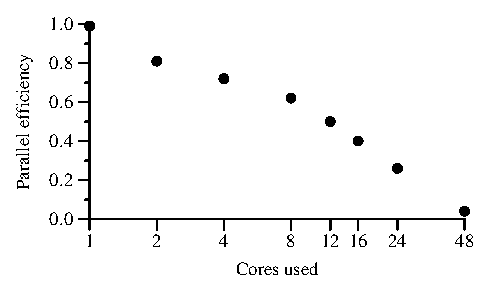
\includegraphics{efficiency}}
% \bigskip
% Beautiful $\frac 1 {\log p}$!
% \caption{\mrfy's parallel efficiency}
% \label{fig:speedup}
% \end{figure}




\end{document}
